\chapter{Background Estimation: $\Rcs$ Method}
\label{chap:Rcs}
\minitoc
When searching for new physics, it is important to know precisely the standard model background contributions in the search regions (SRs) explained in the previous chapter. The modeling of the SM is not trivial due to complicated processes such as QCD and lack of well-studied detector performance.
Therefore, simulated samples can be beneficial to have an initial idea on the kinematics. However, they can not be entirely trustful. In this analysis, a data-driven approach is used to estimate the main backgrounds.
To predict the number of events in search regions, the control regions are used with transfer factors, which is called $\Rcs$, measured in lower jet multiplicity regions in data. This is the core background estimation method of the analysis. 
$\Rcs$ is defined as the ratio of number of events in SR to the number of events in CR:\\
\begin{equation}
\label{eq:rcs}
R_{CS} = \frac{N(\Delta\Phi>x)}{N(\Delta\Phi<x)} = \frac{N^{SR}}{N^{CR}}.
\end{equation}
$\Rcs$ is measured in lower $\njet$ regions, which are not overlapping with the search regions. This requires that the $\Rcs$ values are stable as a function of $\njet$. 
Throughout this thesis, these regions are called as side band regions (SB). The formulation of this procedure is:
\begin{equation}
\label{eq:RcsProc}
{N_{MB}^{SR}} = {R_{CS}^{MB} \cdot N_{MB}^{CR}},\\
{R_{CS}^{MB} \sim R_{CS}^{SB}},\\
{N_{MB}^{SR}} = {R_{CS}^{SB} \cdot N_{MB}^{CR}}.\\
\end{equation}
Requiring no b-tagged jets in the final state leads to both $\wJets$ (see Sec. \ref{sec:RcsW}) and $\ttJets$ (see Sec. \ref{sec:RcsTT}) background components to be equally important in the MB SR.  Other small background contributions are less than 10\% and directly taken from the MC. 
Consequently, the predicted number of events in main band signal regions can be written as the sum of its components:
\begin{equation}
\label{eq:rcss}
N_{Total}^{SR} = N_{\wJets}^{SR}+N_{\ttJets}^{SR}+N_{other}^{SR(MC)}.
\end{equation}
The $\Rcs$ strategy developed for this analysis takes into account the differences in $\Rcs$ values of these two components.
Furthermore, the $\Rcs$ can be defined as a combination of $\Rcs$ from different source of backgrounds:
\begin{equation}
\label{eq:rcs_frac}
R_{CS} = \frac{N^{SR}}{N^{CR}} = \frac{\sum N^{SR}_i}{N^{CR}} = \sum \frac{ N^{SR}_i}{N^{CR}} \cdot \frac{ N^{CR}_i}{N^{CR}_i} = f^{CR}_i \cdot R_{CS}^i,
\end{equation}
where i stands for either $\wJets$ or $\ttJets$ and $f^{CR}_i$ is the relative yield of the ith background component. 
The relative compositions in low $\DF$ control regions are determined from fit to data (see Sec. \ref{sec:bkgcomp}). The measurement of $\Rcs$ is performed in two seperate side band regions. These regions are chosen, such that they mimic the kinematics of the main band as closely as possible.
For $\ttJets$, the side band region is $4\leq\njet\leq5$ and $\nbjet\geq1$ while for $\wJets$ the side band is chosen as $3\leq\njet\leq4$ and $\nbjet=0$.
Despite the fact that QCD multijet events have low contribution in main band signal regions, their contemination in side bands as well as the control regions of main bands has to be estimated and subtracted prior to application of the $\Rcs$ method. Again a data based approach is used (see Sec. \ref{sec:QCDest}).
Tab. \ref{tab:SBMBRegions} summarises the main band and side band regions used in this analysis.
The background prediction mechanisms are validated with data as described in Sec. \ref{sec:Val}.
\begin{table*}[!htb]
\caption{Overview of the definitions of sideband and mainband regions.
For the multijet (QCD) fit the electron (e) sample is used, while for the determination (det.)
of $\Rcs(\wJets)$ the muon ($\mu$) sample is used. Empty cells are not used in the analysis.
}
\label{tab:SBMBRegions}
\centering
\begin{tabular}{c|c|c}
$\nbtag$       & $\nbtag = 0$                                    &  $\nbtag\geq1$\\ \hline
$\njet=3$      &  $\Rcs(\wJets)$ det. ($\mu$ sample)& \\ \cline{1-1}  \cline{3-3}
$\njet=4$      &  QCD bkg. fit (e sample)  & \multirow{2}{*}{$\Rcs(\ttJets)$ det.} \\\cline{1-2}
$\njet\geq5$ & Main band regions &  \\ \hline
\end{tabular}
\end{table*}
%In Figure \ref{fig:rcsMC}, the $\Rcs$ values are shown as a function of $\njet$ for $\wJets$ (left) and $\ttJets$ (right). These figures are presenting only simulated $\Rcs$ values. They suggest the $\Rcs$ values are stable but different for  $\wJets$ and $\ttJets$. Therefore, the $\Rcs$ method is applied to these two background samples separately: $\wJets$ (see Sec. \ref{sec:RcsW}) and $\ttJets$ (see Sec. \ref{sec:RcsTT}). 
%\begin{figure*}[!hbt]
%    \begin{center}
% 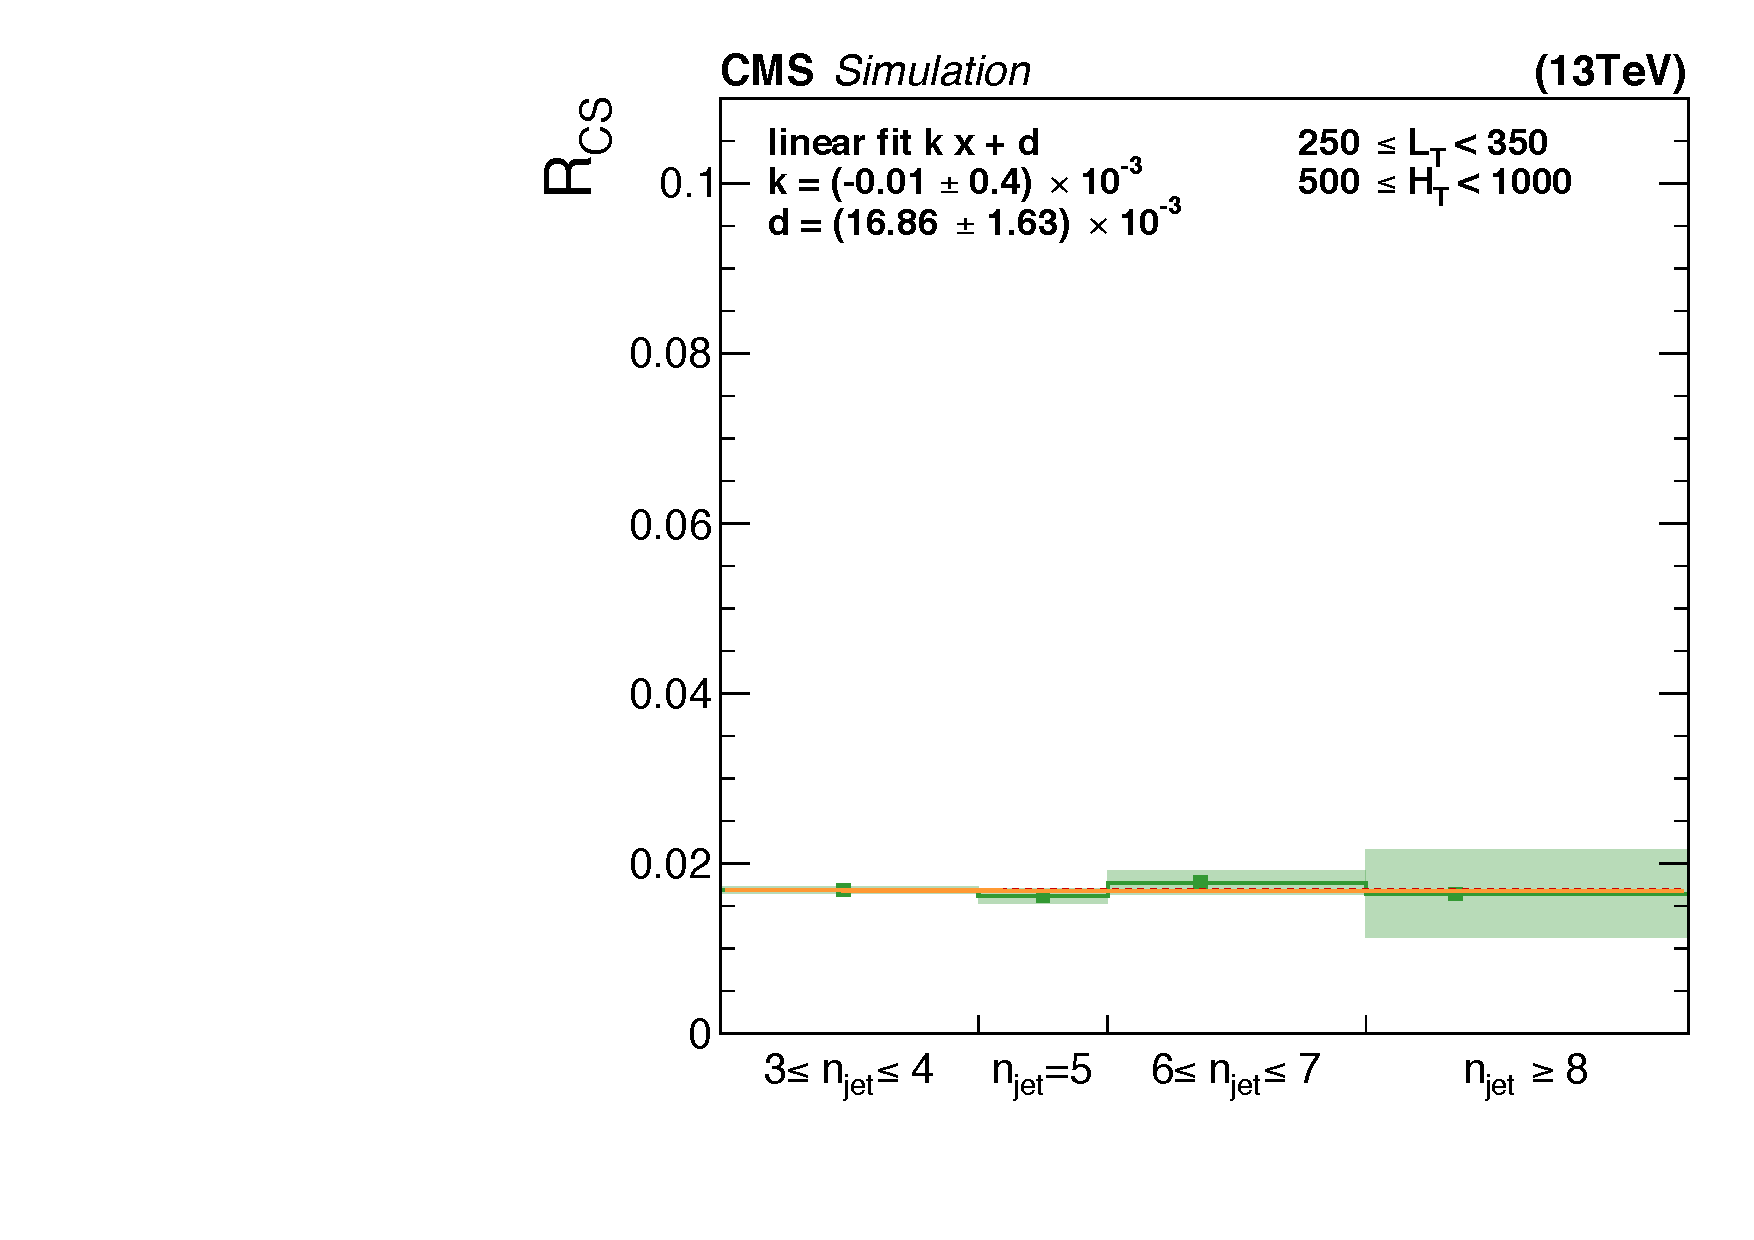
\includegraphics[width=0.45 \textwidth]{Plots/analysis/RCS/st250-350_ht500-1000_njet8_nbtag0_Wjets_NegPdg_fit}
% 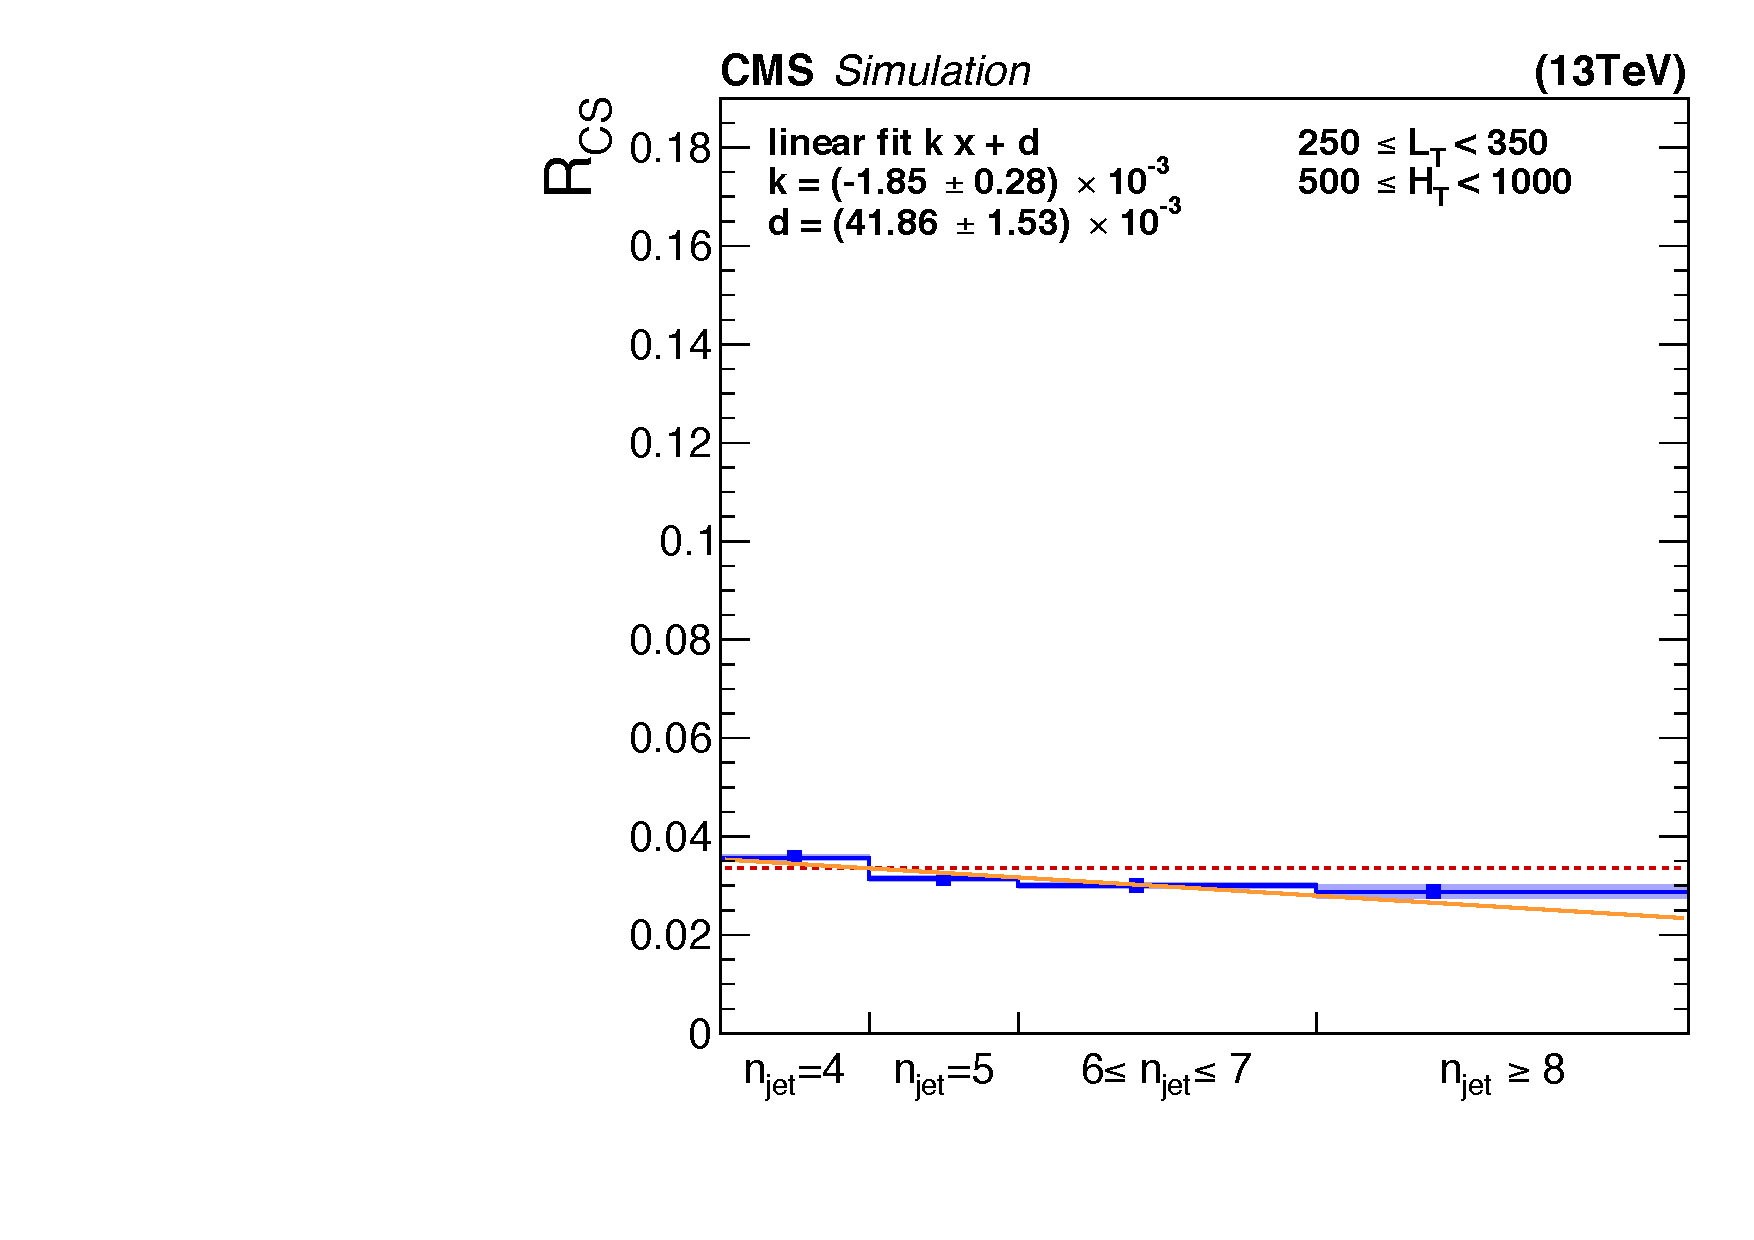
\includegraphics[width=0.45 \textwidth]{Plots/analysis/RCS/st250-350_ht500-1000_njet8_nbtag0_ttjets_all_fit}
%  \caption{ \label{fig:rcsMC} $\Rcs$ distributions as a function of $\njet$ for $\wJets$ (left) and $\ttJets$ (right) simulated events. Distributions belong to $\LT$ [250,350] GeV , $\HT$ [500,1000] GeV bin. 
% }
%  \end{center}
%\end{figure*}
%Residual differences between the $\Rcs$ in the SM and MB is calculated in simulation as a correction factor $\kappa$. Then, the predicted event counts are  corrected with this factor. For this analysis, two $\kappa$ factors for $\wJets$ and $\ttJets$ are evaluated and these will be explained in the following dedicated sections. 
%The QCD multi-jet background is estimated in a fake-lepton enriched data sample and it is introduced in section \ref{sec:QCDest}.  
\section{QCD background estimation}
\label{sec:QCDest}
Due to the complicated nature of quantum chromodynamics (see Sec. \ref{sec:StandardModelParticleInteractions}), simulation of QCD multi-jet events is challenging and fails to be accurate. Naturally in this case, a data-driven prediction of the QCD events in search regions is necessary.
According to simulation, the majority of the QCD multijet events are located in CRs and side band (low $\njet$) regions.
Although, QCD multijet events are not one of the main backgrounds, in order to have a more accurate calculation of $\Rcs$, this contamination needs to be subtracted from SBs and as well as the CRs of MBs. Therefore, the prediction of QCD multi-jet events has to be performed prior to the $\Rcs$ method.\\
Involvement of QCD events in signal regions occurs through fake leptons, which are misidentified jets or photons. Thus, a fake-lepton enriched data control sample, which is obtained by loosening and inverting the criteria on lepton identification variables, is designed for the estimation. To estimate the fraction of events with fake leptons, that pass the analysis selection, ratio of selected to anti-selected events ($F_{\rm sel}$) is used. To ensure the orthogonality to the main band regions, this ratio is measured in $3\leq\njet\leq4$ and $\nbjet=0$ side band. The feature of containing fake leptons helps also to distinguish QCD events from the EWK ones (containing real leptons) by using a variable which reflects the polarisation of the $W$ boson. A variable called $\LP$ was introduced in \cite{LP}, it was for the first measurement of the $W$ polarization at LHC.
The variable $\LP$ is defined as follows:
\begin{equation}
\label{eq:LP}
{\LP} = \frac{\ptvec(\ell)\cdot\ptvec(W)}{|\ptvec(W)|^2} = \frac{\pt(\ell)}{\pt(W)} \rm cos(\DF(W,\ell)),
\end{equation}
where $\ptvec(\ell)$ and $\ptvec(W)$ are the transverse momenta of the charged lepton and the $W$ boson respectively. 
As seen in Fig. \ref{fig:QCD}, QCD events (dashed cyan colored lines) mostly populate the $\LP$ around 1 while the EWK events has a falling distribution between 0 to 1. The number of QCD events in the control regions for selected leptons is then obtained by multiplying the yield of the anti-selected events, which is obtained from the example template fit shown in Fig. \ref{fig:QCD} (left), with $F_{\rm sel}$ which is shown in the same figure as a function of $\LT$ bins.\\
A profound description of the method can be found in \cite{David}.
\begin{figure*}[!hbt]
    \begin{center}
 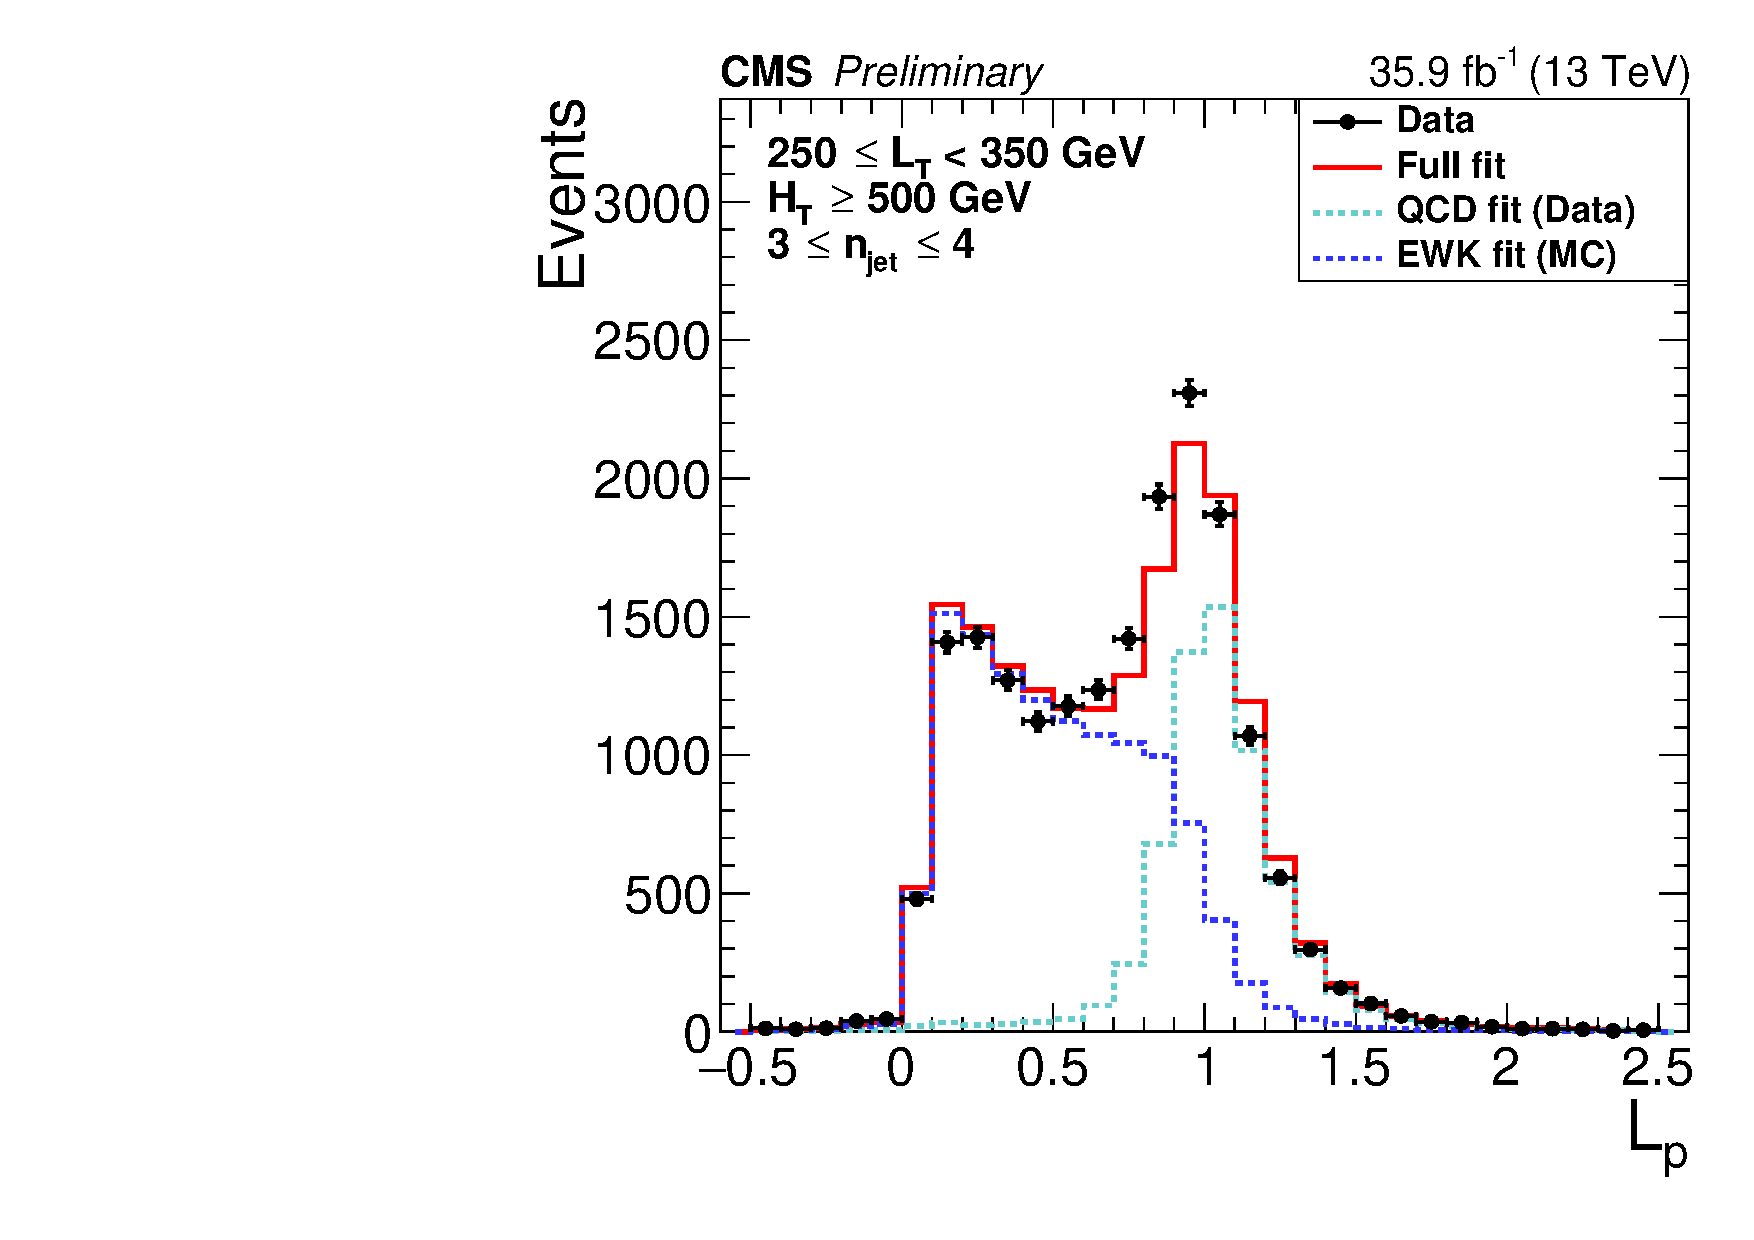
\includegraphics[width=0.45 \textwidth]{Plots/analysis/QCD/Lp_singleElectronic_st250-350_ht500_njet3-4_nbtagEq0_TemplateFit.pdf}
 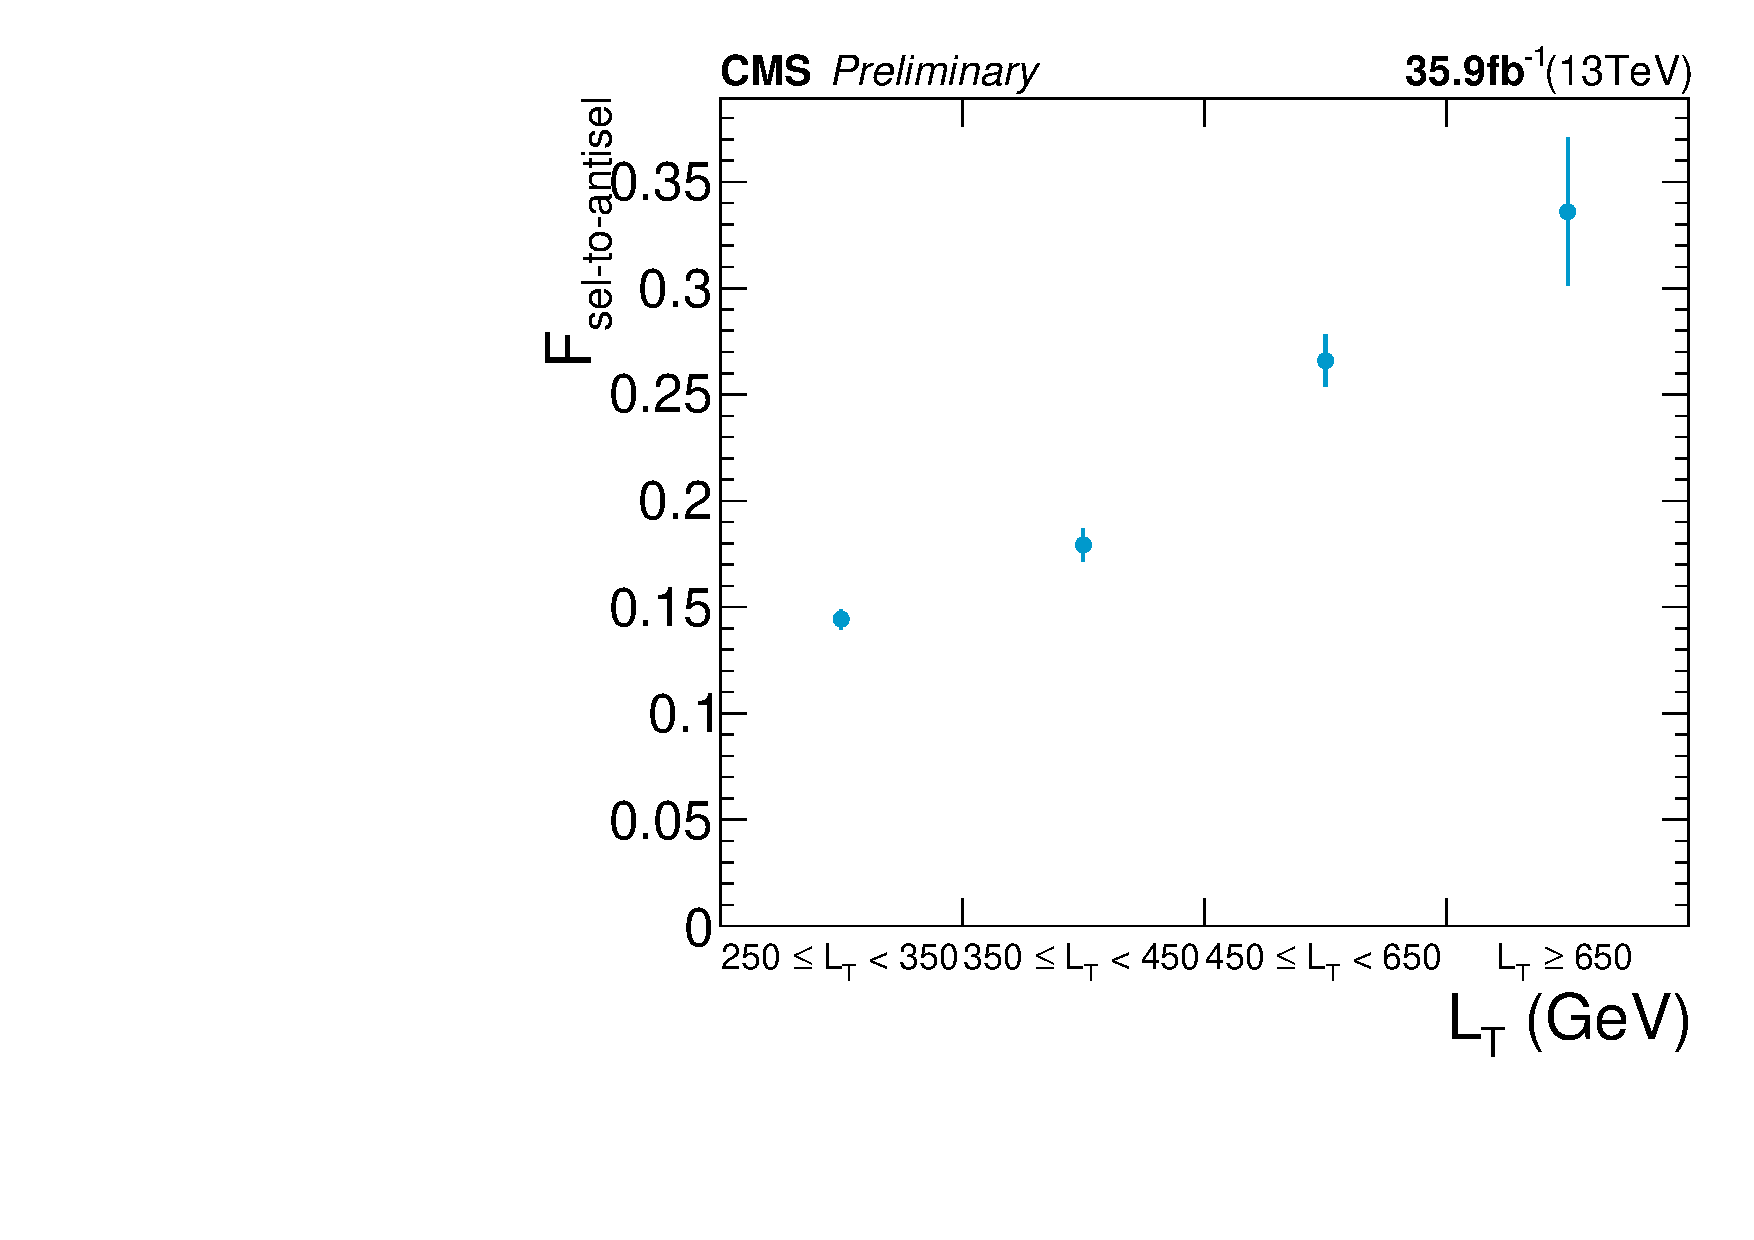
\includegraphics[width=0.45 \textwidth]{Plots/analysis/QCD/Fsel.pdf}
  \caption{ \label{fig:QCD} $\LP$ shape fit result for $3\leq\njet\leq4$ and $\nbjet=0$ in $250\leq\LT\leq350$ bin (left).  Ratio of selected to anti-selected electron events from QCD for $3\leq\njet\leq4$ and $\nbjet=0$, in bins of LT in data (right). 
 }
  \end{center}
\end{figure*}
\section{Background fraction calculations: b-tag multiplicity fit}
\label{sec:bkgcomp}
Fractions of the background processes in the control regions ($f^{CR}_i$) are calculated using likelihood fit of b-tag multiplicity distributions templates to data. The templates are obtained from simulation except the QCD events. The QCD multijet contribution in b-tag multiplicity bins is taken from the prediction, which is introduced in the previous section. \\
$\wJets$ events display a charge asymmetry in $\Rcs$ due to polarization effects. To account for this, the fits are performed separately for each charge: positive and negative.
$\ttJets$ and QCD events are considered as homogenous in charge. Other background templates are also produced separately for positive and negative charged leptons. 
Fig. \ref{fig:btagmult} shows good agreement between data and the b-tag multiplicity fit.
\begin{figure*}[!hbt]
    \begin{center}
 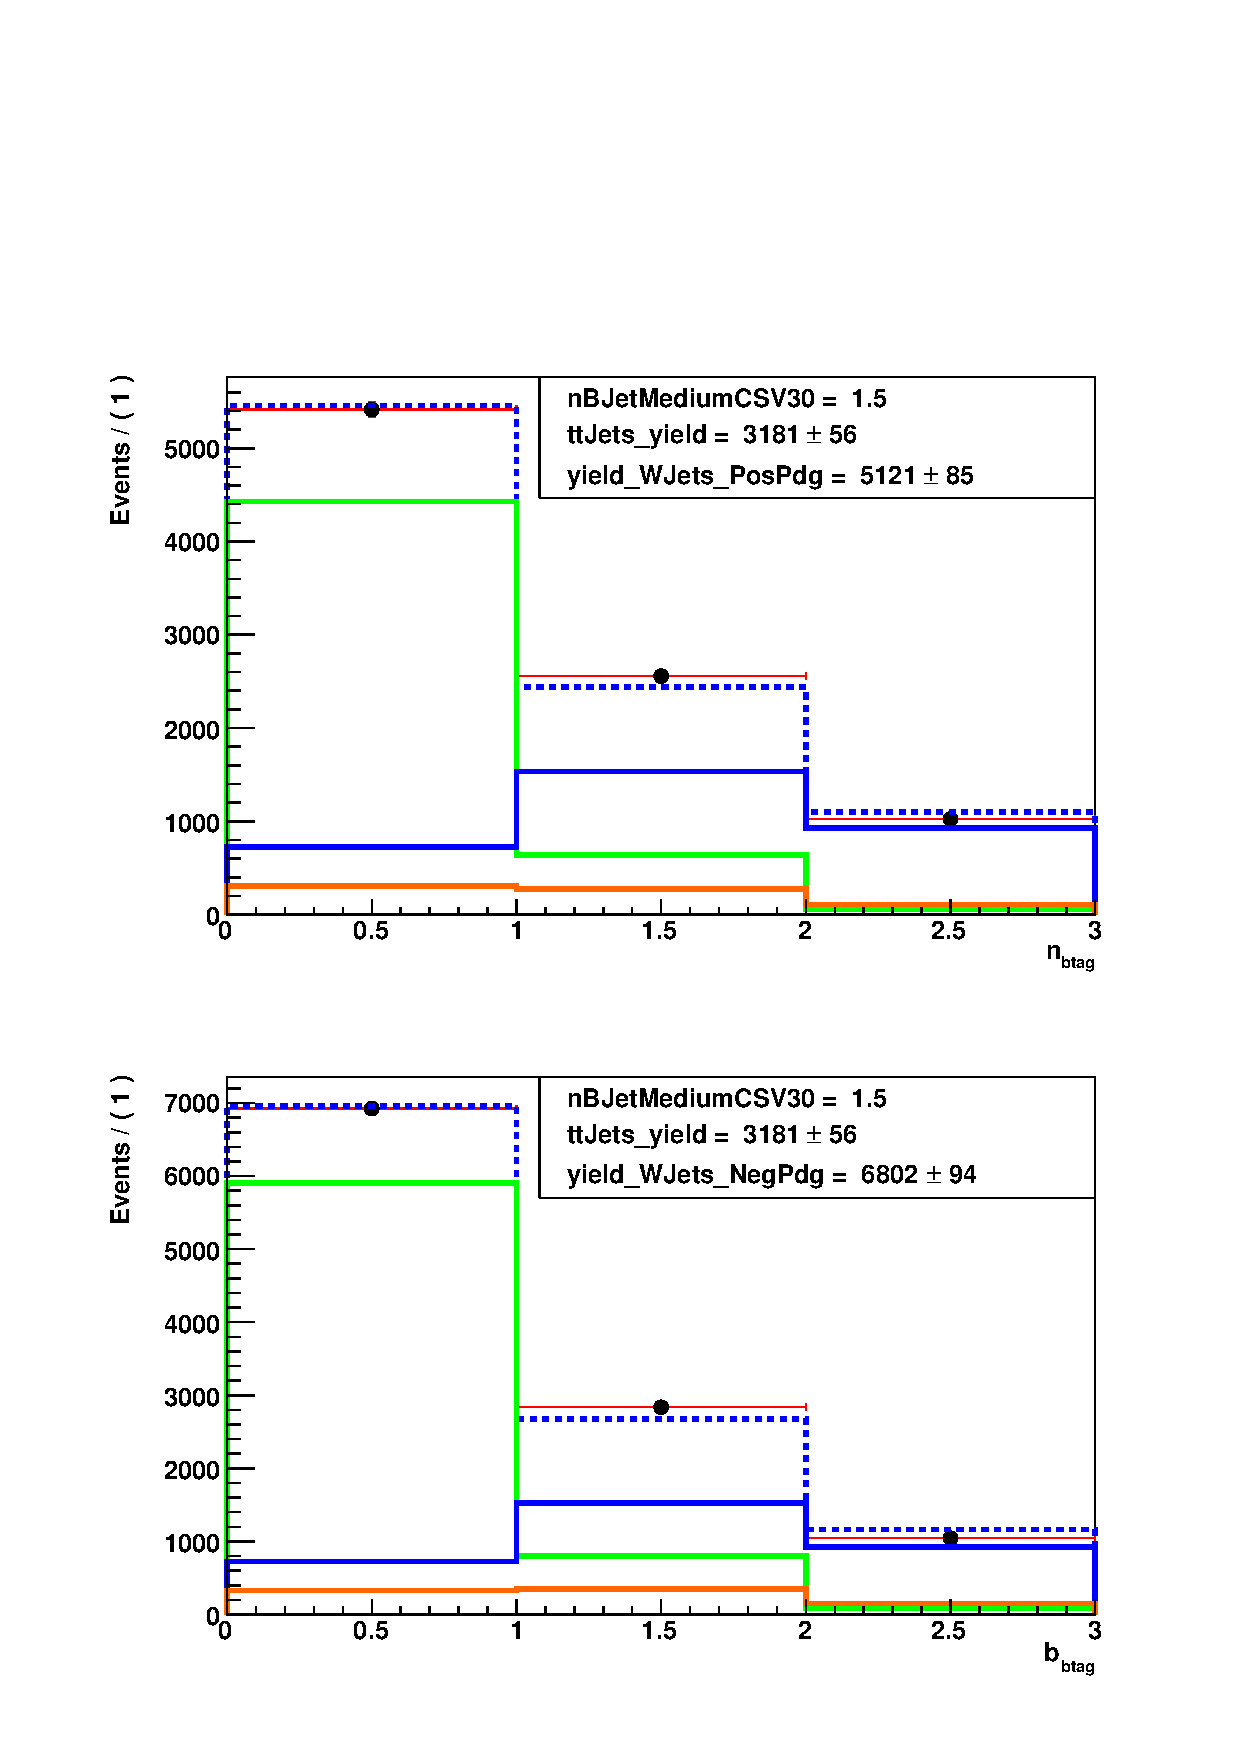
\includegraphics[width=0.48 \textwidth]{Plots/analysis/signalRegions/34jets}
 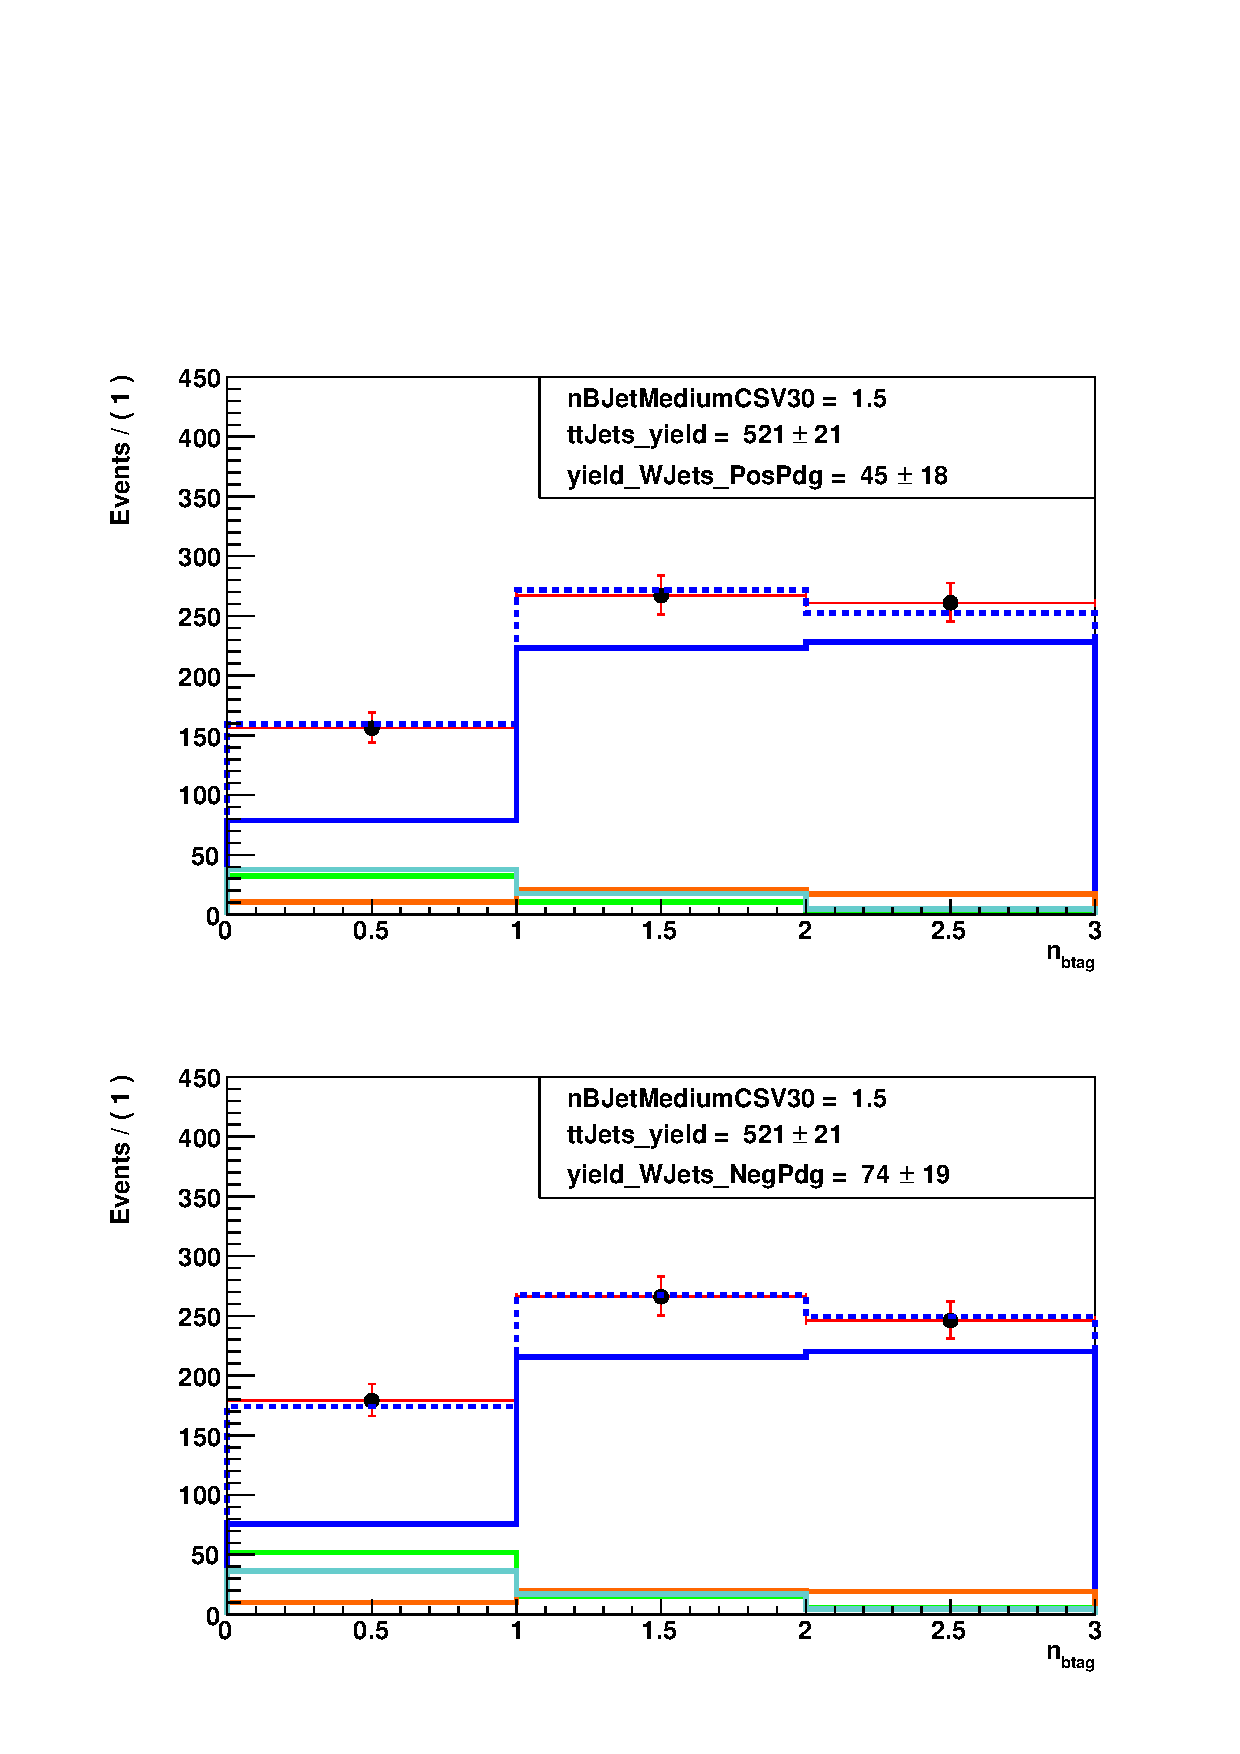
\includegraphics[width=0.48 \textwidth]{Plots/analysis/signalRegions/8jets}
  \caption{ \label{fig:btagmult} b-tag multiplicity fit is performed in control regions. 3-4 jets sideband (left), 8 jets main band (right). Upper plots are showing the negative charged lepton selection while lower plots show the positive charged selection. Balck points represent data, green is for $\wJets$ , blue is for $\ttJets$ , orange is for other EWK backgrounds and  cyan colored lines show QCD contemination.
 }
  \end{center}
\end{figure*}
\section{$R_{CS}$ method in $\ttJets$ events}
\label{sec:RcsTT}
In LHC, the top quark pair production mechanism is dominated by gluon-gluon fusion and quark-quark annihilation. According to the SM, the top quark decays into $Wb$ in almost 100\% of the cases.  In other words, nearly all of the $\ttJets$ events involve two b-tagged jets. However, the b-tagging algorithms are not fully efficient; therefore $\ttbar$ events can survive after the b-tagged jet veto requirement. The surviving events have a very similar final state with the T5qqqqWW signal events. Due to its high cross section,  $\ttJets$ is one of the two main backgrounds of this search. \\
The $\ttbar$ decay can be categorized into three with respect to lepton content of the final state; single leptonic, di leptonic and fully hadronic. The branching ratios of these decay modes are approximately 45\%, 9\% and 44\%, respectively.  After the baseline selection of the analysis, the single leptonic decay channel, where one of the two $W$ bosons decays leptonically, populates the low $\DF$ region while the di leptonic decay channel, where one of the leptons are lost due to misidentification or limited detector acceptance dominates the high $\DF$ region. As a result of this, di leptonic $\ttbar$ events have higher $\Rcs$ values. Fig. \ref{rcsMCtt}  shows the $\Rcs$ as a function of $\njet$ for di leptonic (left) and single leptonic (right) decays separately.
\begin{figure*}[!hbt]
    \begin{center}
 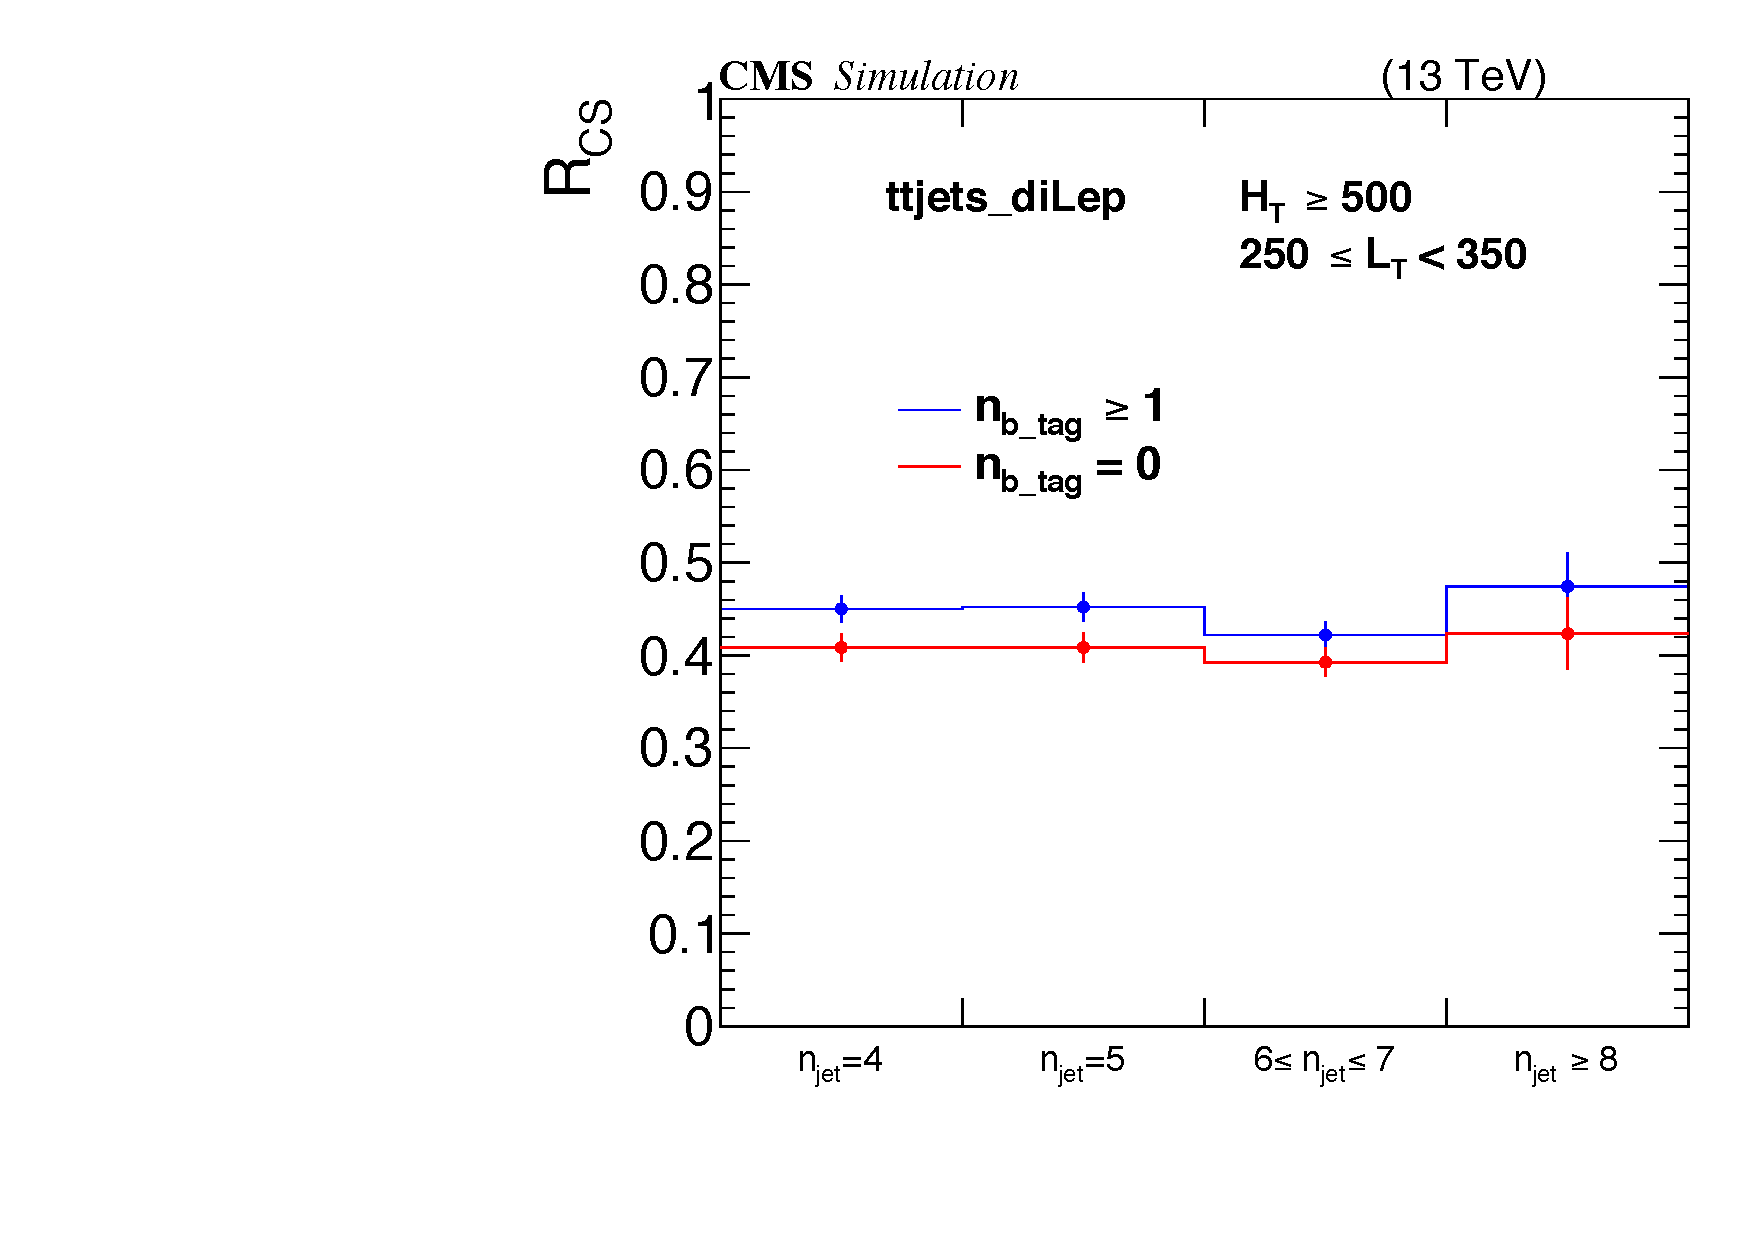
\includegraphics[width=0.45 \textwidth]{Plots/analysis/RCS/dilep}
    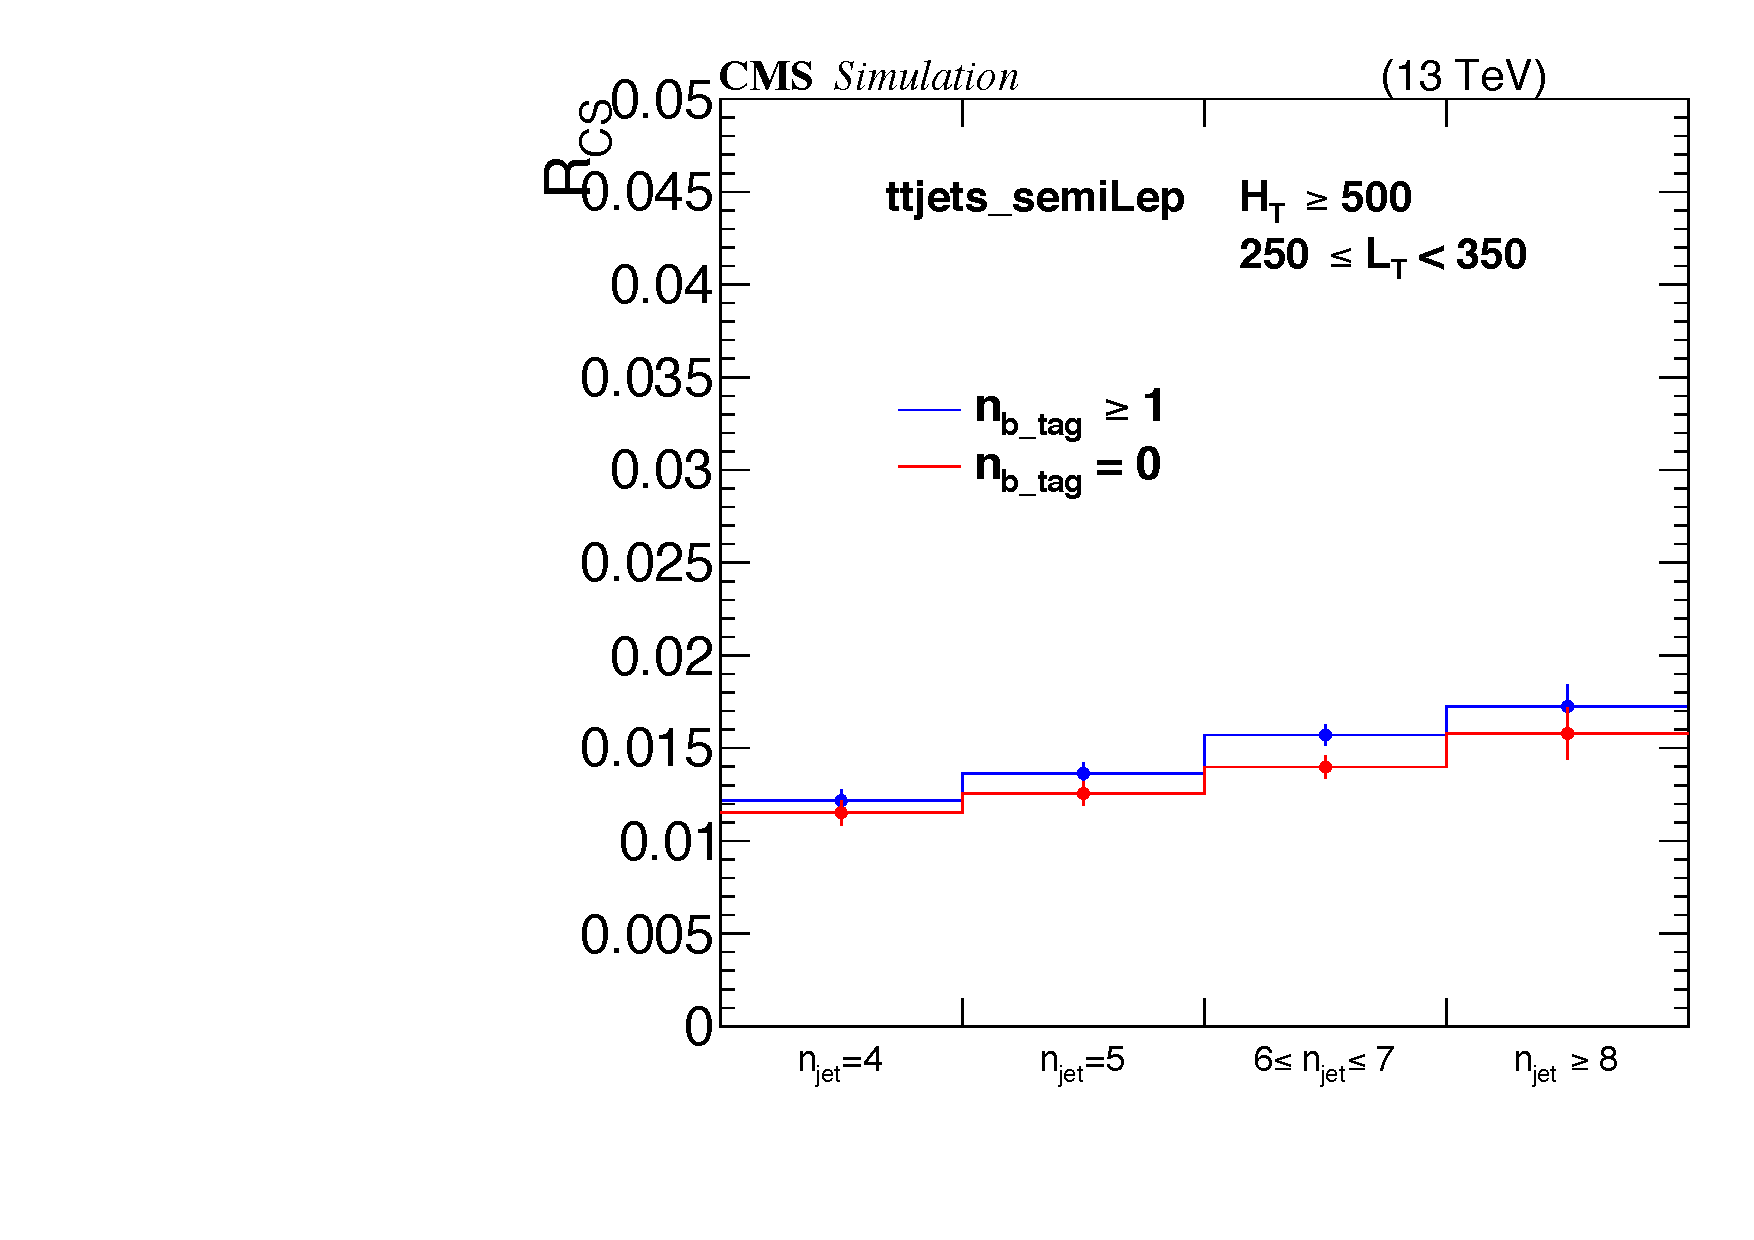
\includegraphics[width=0.45 \textwidth]{Plots/analysis/RCS/semilep}
  \caption{ \label{rcsMCtt}  RCS as a function of njet for dileptonic (left), and signle leptonic (right) tt + jets events. }
  \end{center}
\end{figure*}
It should be noted that this figure shows only simulated values and it is only for illustration.
In the primary background estimation procedure, $\Rcs$ values of $\ttJets$ events are measured in sideband regions requiring four to five jets and at least one b-tagged jet from data. This selection increases the purity of $\ttJets$ events while at the same time keeps $wJets$ events contamination low. In addition to this, the yield of predicted QCD multi-jet events is subtracted from the CR. The formulation of $\Rcs$:
\begin{equation}
\label{eq:rcsTTdata}
R_{CS}^{data}(b \geq 1, \njet \in [4,5] ) = \frac{N_{SR}^{data}}{N_{CR}^{data}-N_{CR}^{QCD(pred)}}.
\end{equation}
Fig. \ref{RCS_dataMCtt} shows simulated (left) and measured(right) values for the first search bin which is $\njet =$5, $\LT \in$ [250,350] GeV and $\HT \in$ [500,1000] GeV. Residual differences between the $\Rcs$ in the side band and main band is calculated in simulation as a correction factor $\kappa$. In $\ttbar$ background estimation two kind of kinds of $\kappa$ corrections are used.
\begin{figure*}[!hbt]
    \begin{center}
 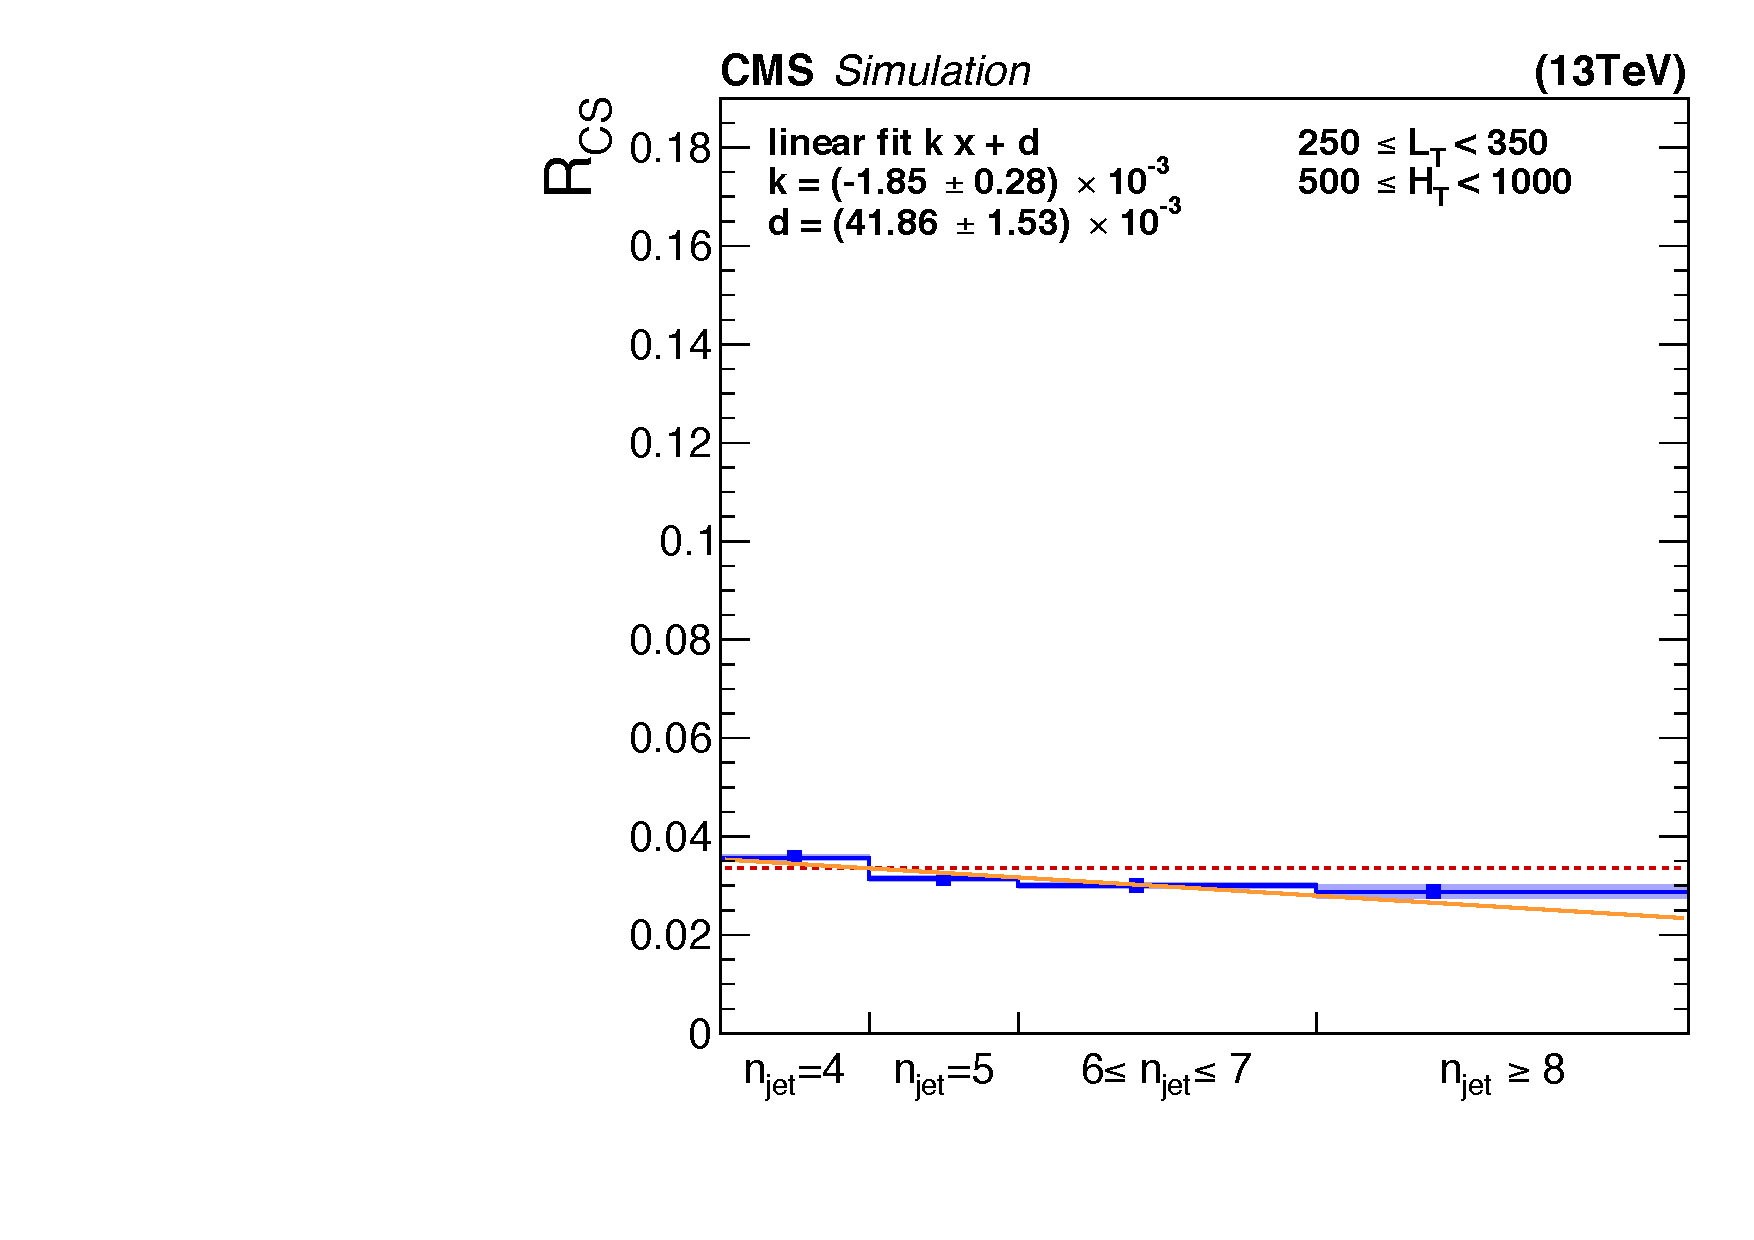
\includegraphics[width=0.45 \textwidth]{Plots/analysis/RCS/st250-350_ht500-1000_njet8_nbtag0_ttjets_all_fit}
    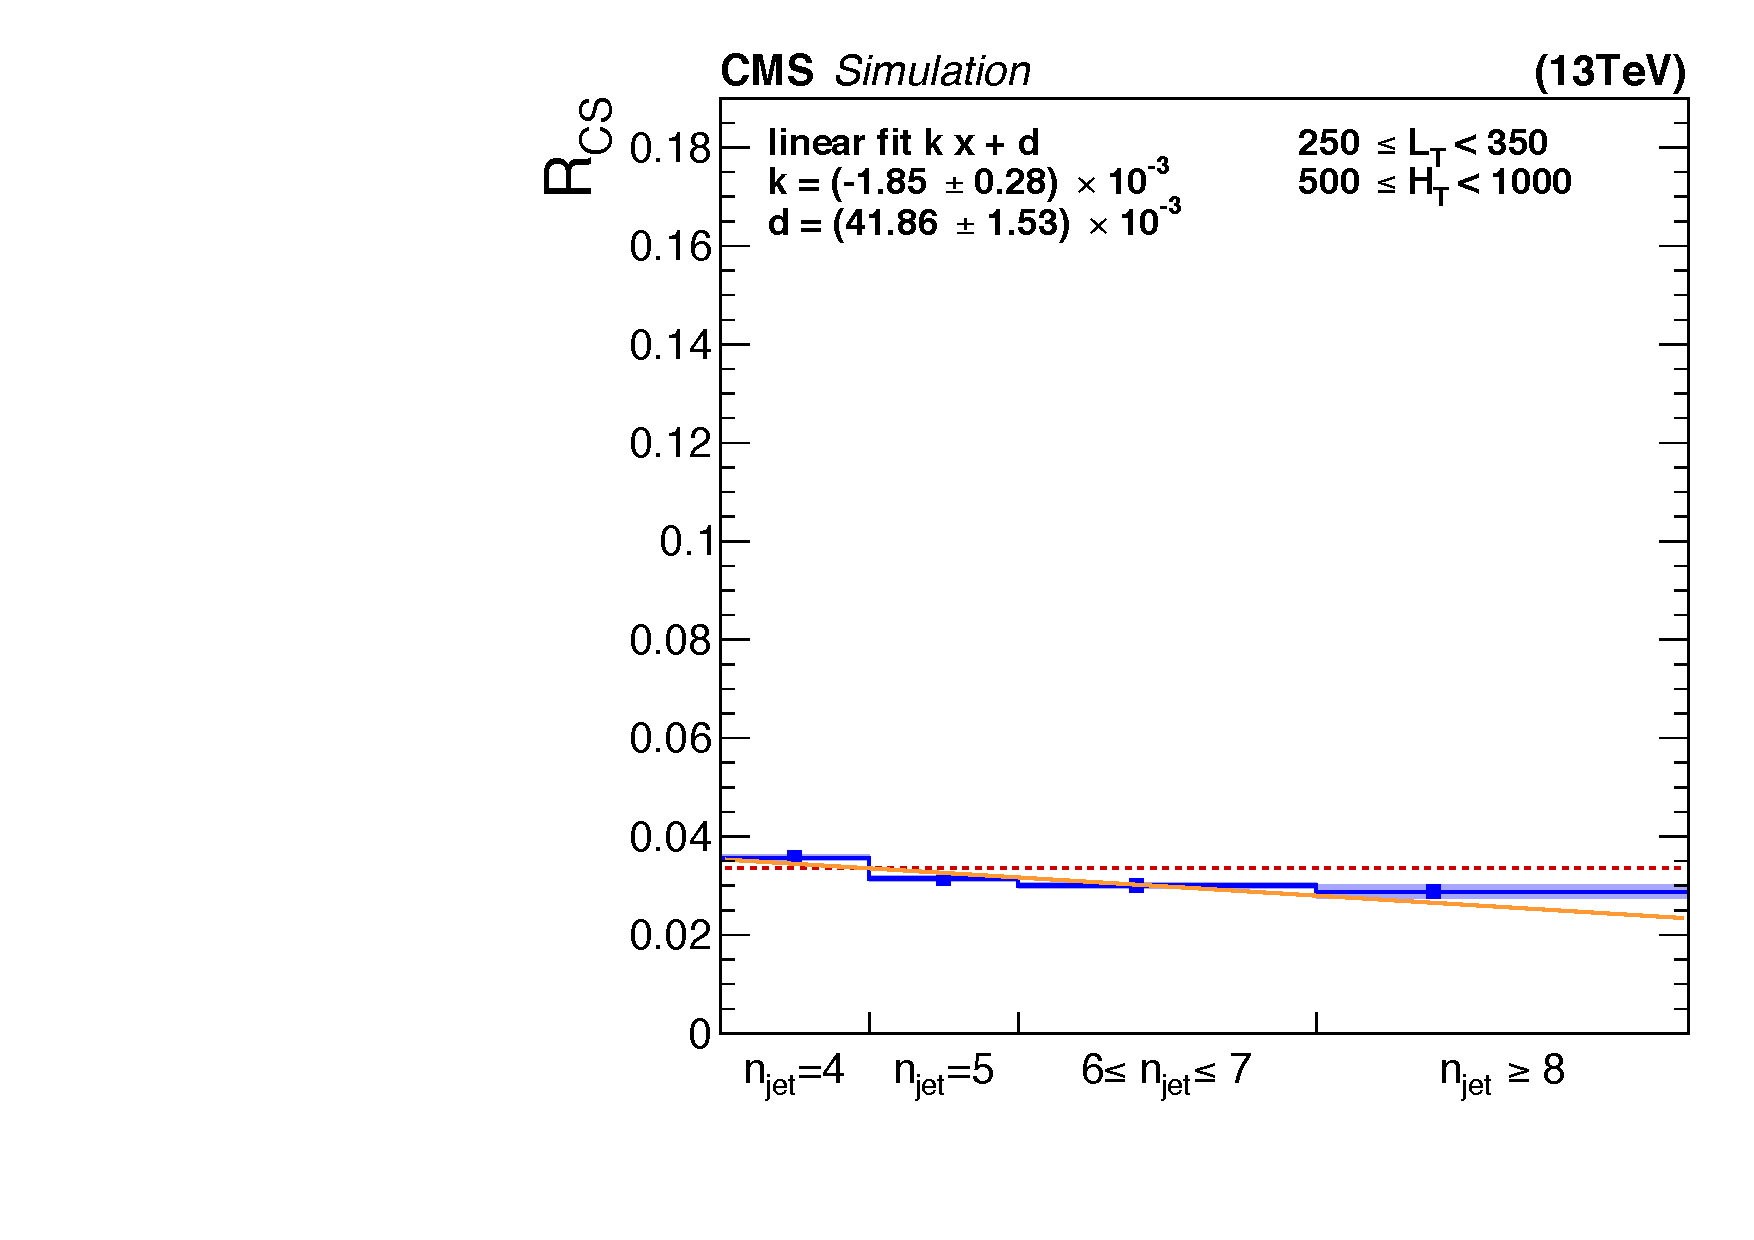
\includegraphics[width=0.45 \textwidth]{Plots/analysis/RCS/st250-350_ht500-1000_njet8_nbtag0_ttjets_all_fit}
  \caption{ \label{RCS_dataMCtt}  $\Rcs$ as a function of njet from simulation of $\ttJets$ events (left), and data (right) in $\ttJets$ sideband. }
  \end{center}
\end{figure*}
The first one is called $\kappa_b$. As the name implies, it covers the possible difference between the $\Rcs$ values of the b-tagged region and no b-tagged region. This correction also accounts for small contributions from processes other than $\ttJets$ and QCD multi-jet. The correction factor $\kappa_b$ can be written as follows:
\begin{equation}
\label{eq:kappaB}
{\kappa_b} = \frac{R_{CS}^{MC}(0b , \njet \in [4,5] , \ttbar )}{R_{CS}^{MC}(b \geq 1 , \njet \in [4,5] , EWK )} 
%{\kappa_b}
\end{equation}
The second correction factor accounts for a residual dependence of $\Rcs$ on jet multiplicity:
\begin{equation}
\label{eq:kappatt}
{\kappa_{\ttbar}} = \frac{R_{CS}^{MC}(0b , \njet: MB , \ttbar )}{R_{CS}^{MC}(0b , \njet \in [4,5] , \ttbar )} 
%{\kappa_b}
\end{equation}
As mentioned in the beginning of this chapter, the total $\Rcs$ is based on the fraction of different channels and their corresponding $\Rcs$ values. In this case, the difference between $\Rcs$ values of single leptonic and di leptonic events should be considered. In this point, another control region is designed to understand the effect of di lepton events that pass the single lepton selection. To obtain a high-purity di lepton $\ttbar$ control sample in data, two leptons of opposite charge are required. It is also required that the mass of two same flavor leptons is more than 10 GeV away from the $Z$ mass peak. To mimic the single lepton events, one of the two leptons is removed. 
These so-called lost leptons are mostly coming from $\tau \rightarrow$ hadrons + $\nu$ decays. Therefore, the removed lepton is replaced by a jet with 2/3 of the original lepton's \pt to account for the missing energy due to the neutrino from the $\tau$ decay.  The $\LT$, $\HT$ and $\DF$ values of the reconstructed single-lepton event are recalculated.
No $\DF$ requirement is applied, and all events are used twice, with each reconstructed lepton being considered as the lost lepton to increase the statistics in this di-lepton control region.
In Fig. \ref{dl-CR}, the top row displays the $\njet$ distributions for the lost lepton events obtained from di lepton ones (left) and usual single lepton events (right) in control region (low $\DF$). The distributions are obtained after baseline requirement for $\LT$ and $\HT$ with a lower jet multiplicity requirement ($\njet \geq 3$) to account for side band regions. The correctness of the description of the $\njet$ distribution in simulation is determined from the double ratio, which is the single-lepton and di lepton ratio between data and simulation, as shown in the bottom of the same figure.
\begin{figure*}[!hbt]
    \begin{center}
 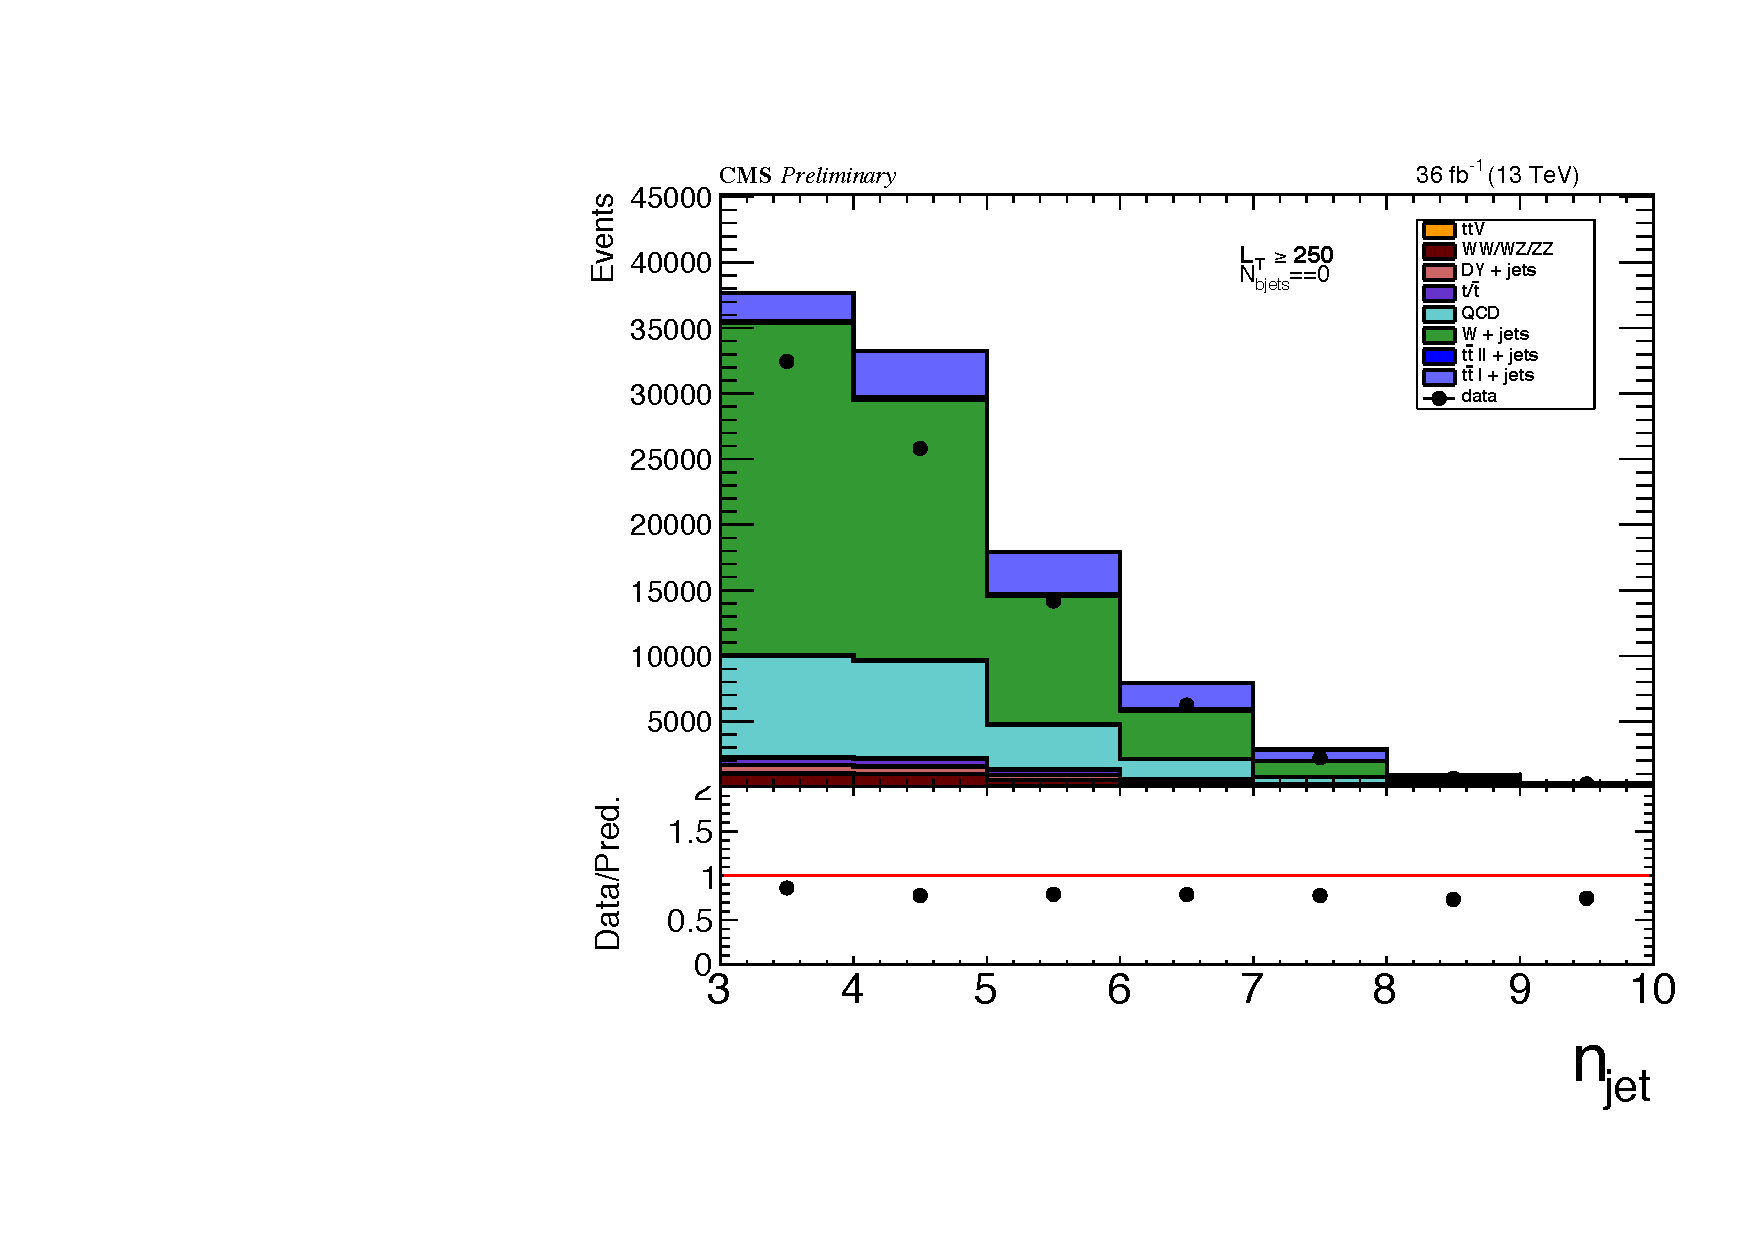
\includegraphics[width=0.4 \textwidth]{Plots/analysis/RCS/diLepCR/singLep}
 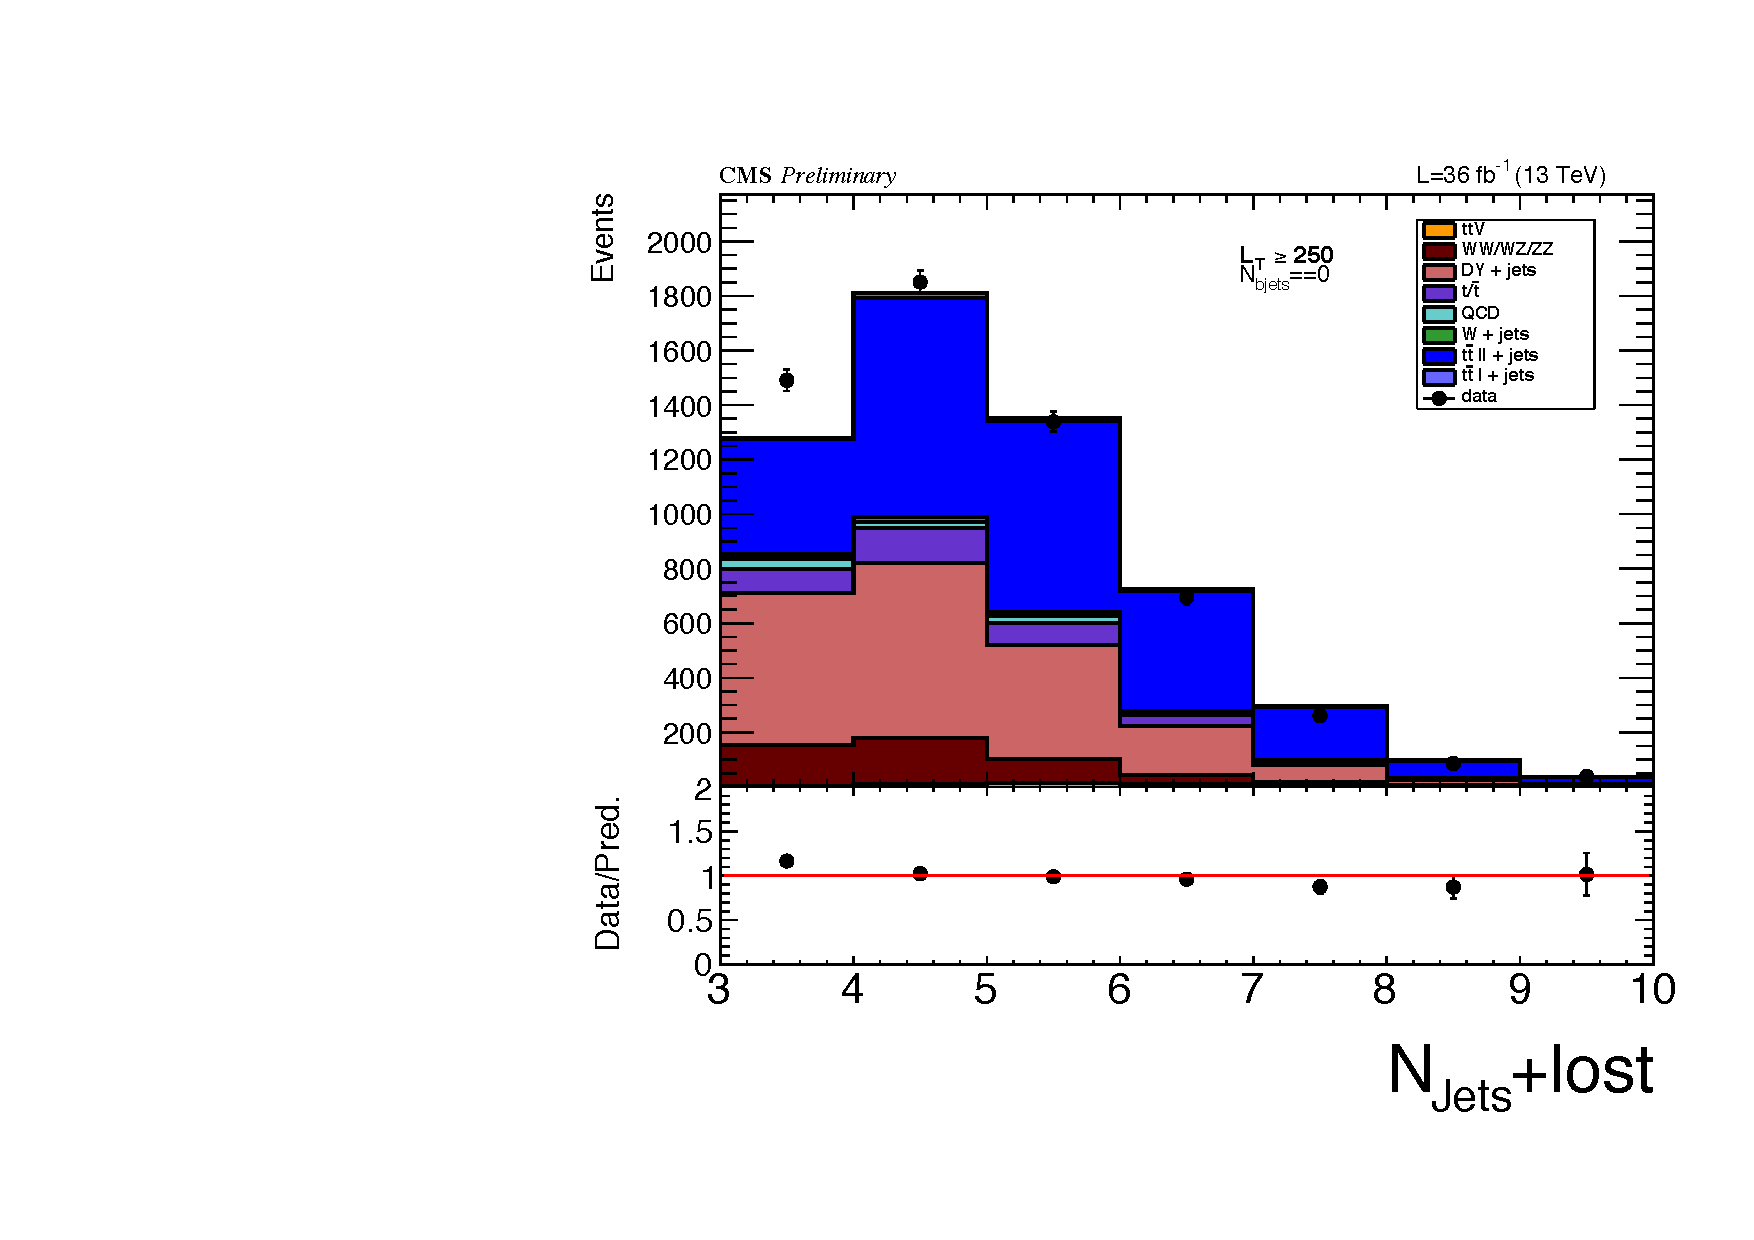
\includegraphics[width=0.4 \textwidth]{Plots/analysis/RCS/diLepCR/diLep}\\
    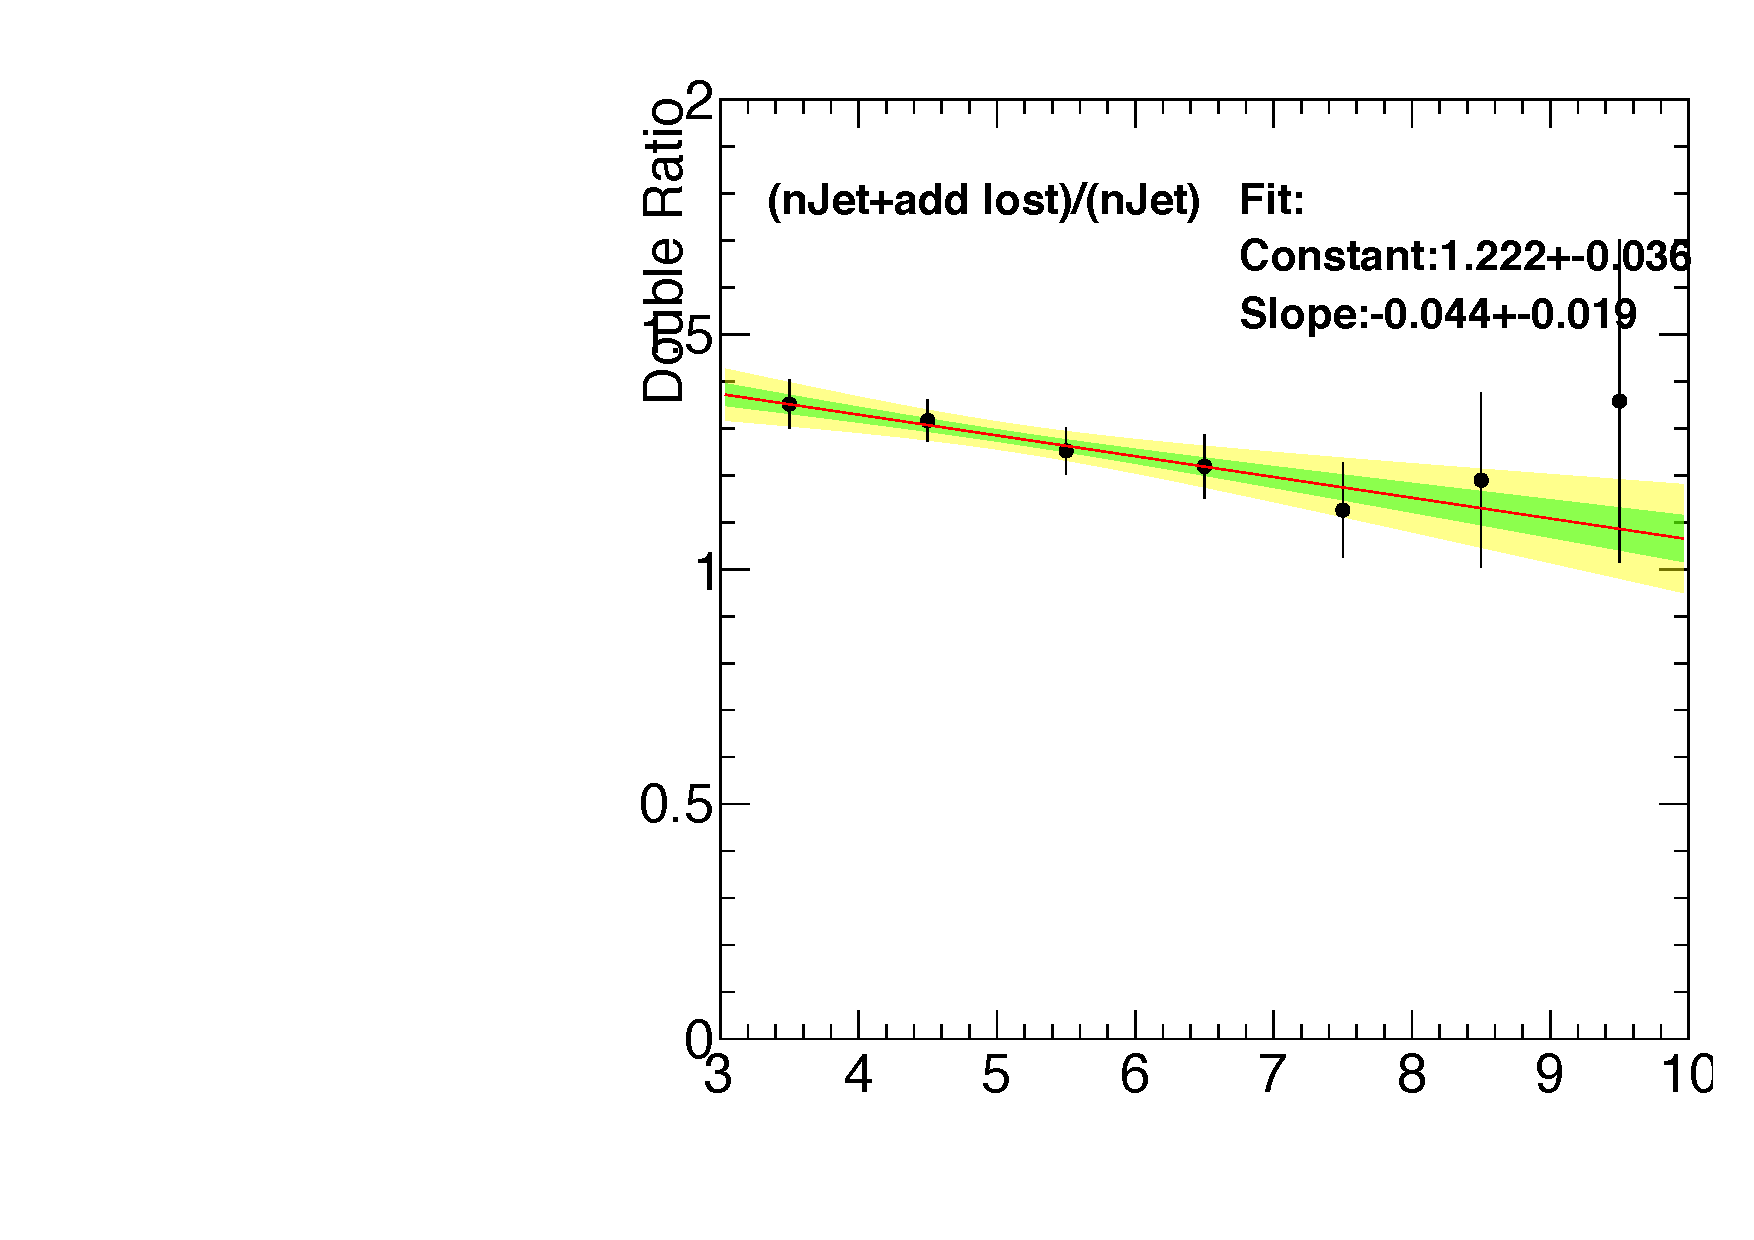
\includegraphics[width=0.4 \textwidth]{Plots/analysis/RCS/diLepCR/double_Ratio}
  \caption{ \label{dl-CR} Jet multiplicity distribution after the single lepton baseline event selection (in the control region)
 with $\HT>500$ GeV, $\LT>250$ GeV, and $\nbtag = 0$ (left) and in the dileptonic control region with recalculated $\HT$ and $\LT$ cuts (right). Only nISR reweighting is applied as scale factors. }
  \end{center}
\end{figure*}
In the case simulation discribes the dileptonic events in data entirely, the double ratio would be flat and located around 1.
However, double ratio manifests that the di leptonic events in simulation should be corrected to calculate a more accurate $\kappa_{\ttbar}$.
The weight for dileptonic events are extracted from double ratio : 
\begin{equation}
\label{weight_DL}
weight_{DL} = 1.22+(-0.044)*(\njet - 5.9),
\end{equation}
where the value 5.9 is coming from the average of the $\njet$ of the single lepton distribution.
The $\kappa_{\ttbar}$ described in Eqn. \ref{eq:kappatt} is replaced with a $\kappa$ calculated after this di lepton correction.
The comparison of $\kappa_{\ttbar}$ before and after correction can be seen in Fig. \ref{fig:kappa_tt}.\\
\begin{figure*}[!hbt]
    \begin{center}
 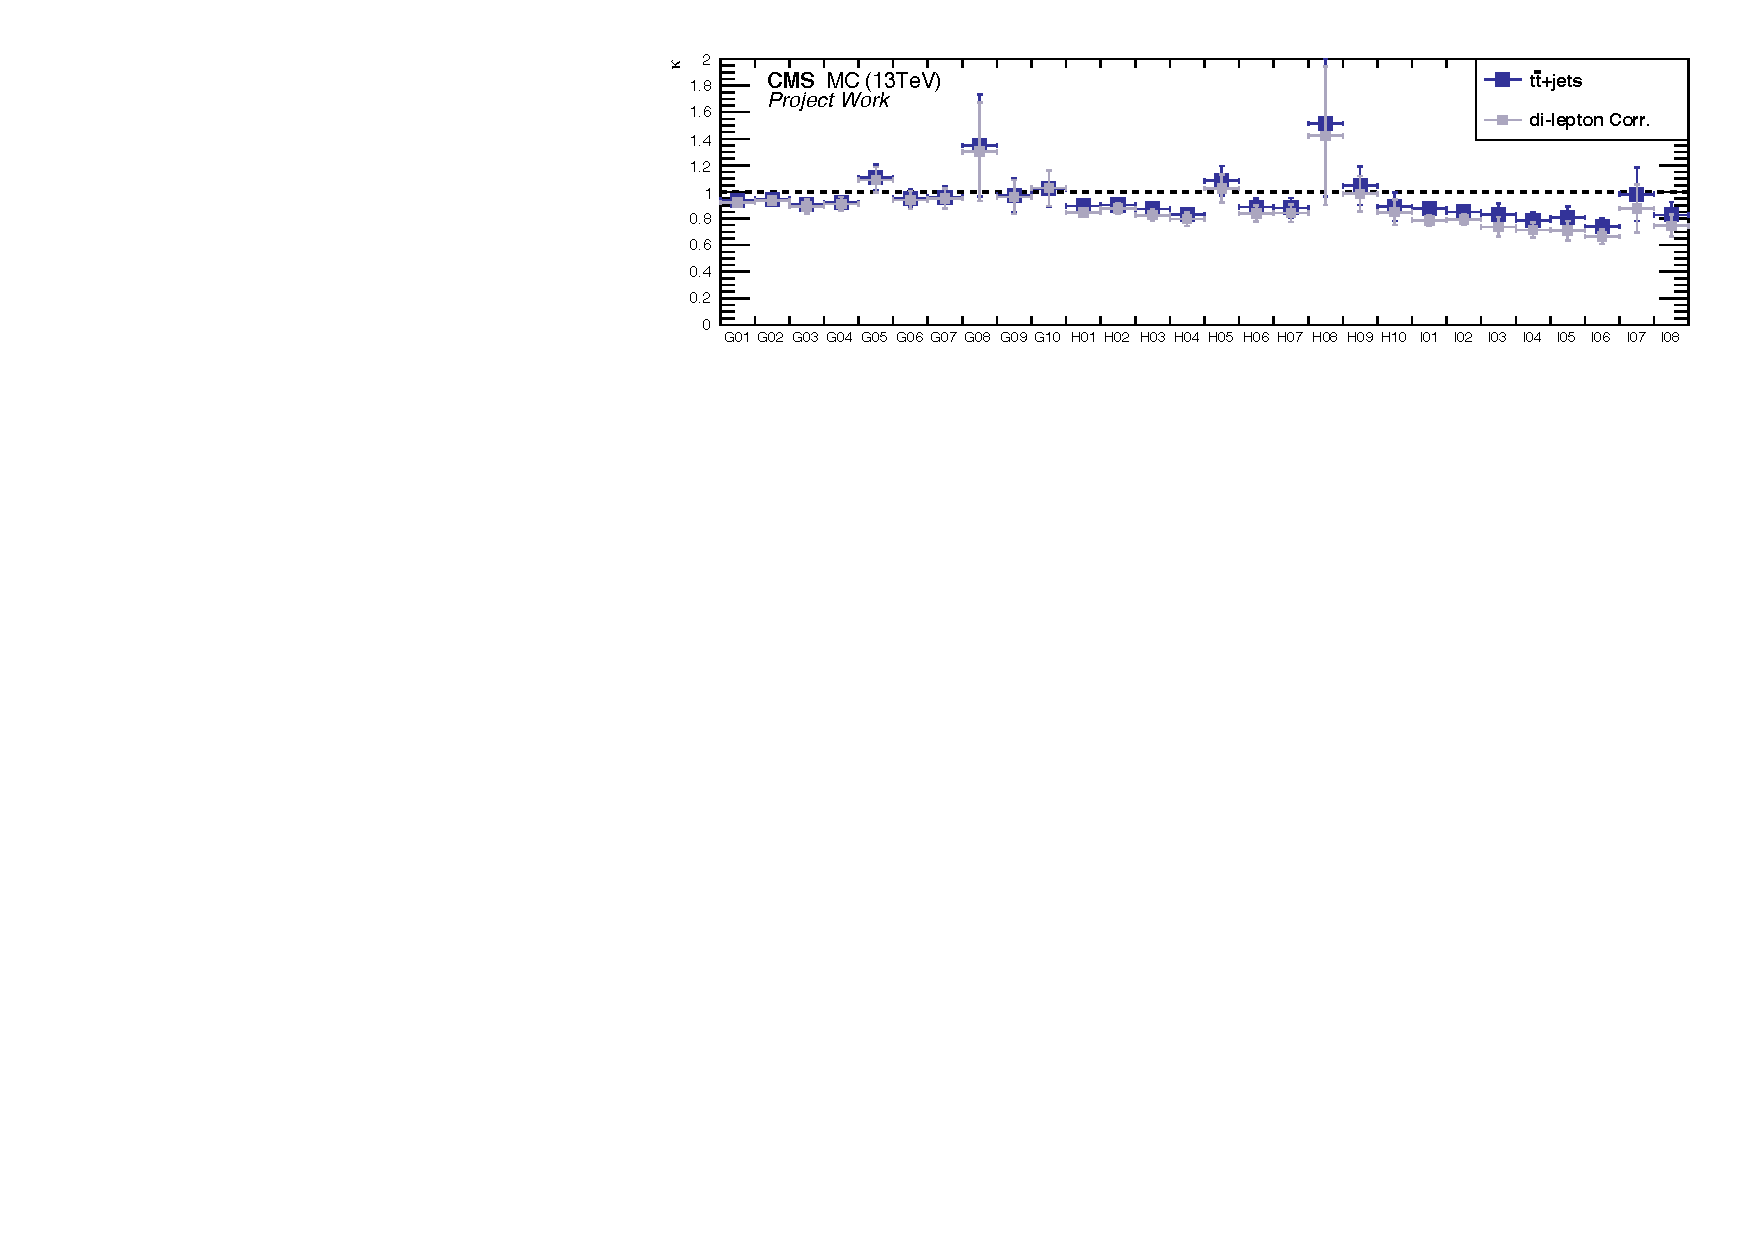
\includegraphics[width=1. \textwidth]{Plots/analysis/RCS/diLepCR/Spring16_templates_SR_Moriond2017_Summer16_lep_data_Kappa_compForthesis}
  \caption{ \label{fig:kappa_tt}  Changes to $\kappa_{\ttbar}$ due to applying the double-ratio as given by Eqn. \ref{weight_DL} and reevaluating $\kappa_{\ttbar}$. The corrected $\kappa$, which is shown with a lighter color, is used as $\kappa_{\ttbar}$ in the full background prediction.}
  \end{center}
\end{figure*}
The resultant $\Rcs$ for $\ttJets$ estimation is then written as:
\begin{equation}
\label{Final_RCS}
R^{\ttbar}_{CS}(0b,MB) = {\kappa_b}\cdot{\kappa_{\ttbar}^{DL-Corr}}\cdot{R_{CS}^{data}(b \geq 1, \njet \in [4,5] )}.
\end{equation}
\section{$R_{CS}$ method in $\wJets$ events}
\label{sec:RcsW}
In this search, when performing the $\wJets$ estimation, the $WV$ di-boson events, where V stands for $W or Z$ bosons, are included in the prediction mechanism. In the di-boson events, which are considered as a part of $\wJets$ estimation, the $W$ boson decays leptonically and the second boson, denoted by V, decays hadronically. The similarity of the kinematics of the events, hence the $\Rcs$ values, makes this addition possible. All other diboson events are treated as part of the rare EWK backgrounds and taken from simulation.\\
$\Rcs$ values for $\wJets$ background estimation is measured in a sideband region with three to four jets. To suppress the $\ttJets$ events and to be kinematically as close as possible to main band regions, zero b-tagged region is used. 
Furthermore, in order to suppress QCD contamination $\Rcs$ is measured only in muon channel. Therefore, it is no longer needed to subtract predicted yield of QCD multi-jet events. However, remaining $\ttJets$ events contamination is subtracted both from signal and control regions. In the determination of the amount of $\ttJets$ events contemination, fractions  $f_{\ttbar}$ in the sideband control region is taken from the b-tag multiplicity fit, and $\Rcs$ is taken from MC directly.
The $\Rcs$ can then be wriiten as:
\begin{equation}
\label{RCSw}
{R^{Corr. data}_{CS}(0b,\njet \in [3,4])} = \frac{N^{SR}_{data}-R^{\ttbar, MC}_{CS}\cdot f^{fit}_{\ttbar}\cdot N^{CR}_{data}}{(1-f^{fit}_{\ttbar})\cdot N^{CR}_{data}}.
\end{equation}
As already disscussed in Sec. \ref{sec:bkgcomp}, $\Rcs$ is separately measured for positive and negative charged leptons to account for the charged asymmetry of the $\wJets$ events. 
\begin{figure*}[!hbt]
    \begin{center}
 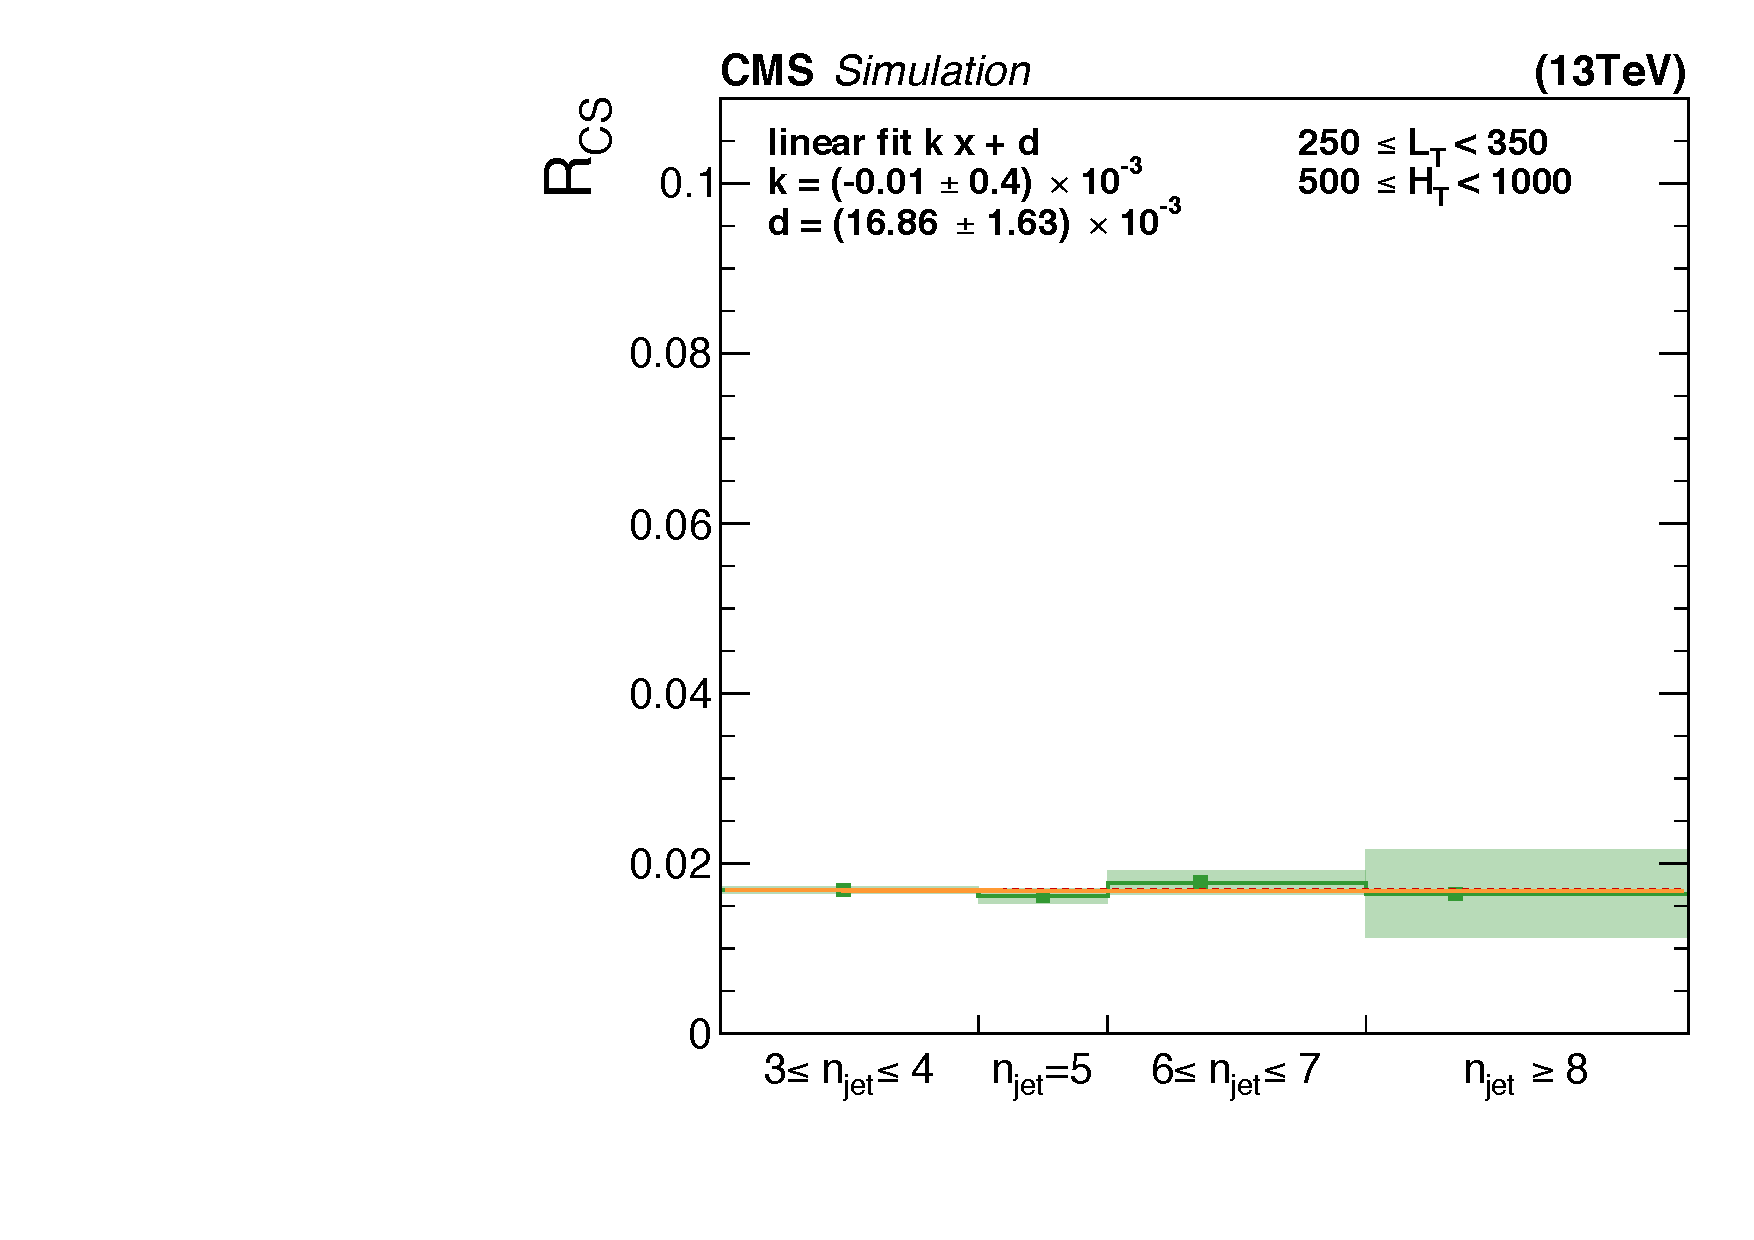
\includegraphics[width=0.45 \textwidth]{Plots/analysis/RCS/st250-350_ht500-1000_njet8_nbtag0_Wjets_NegPdg_fit}
   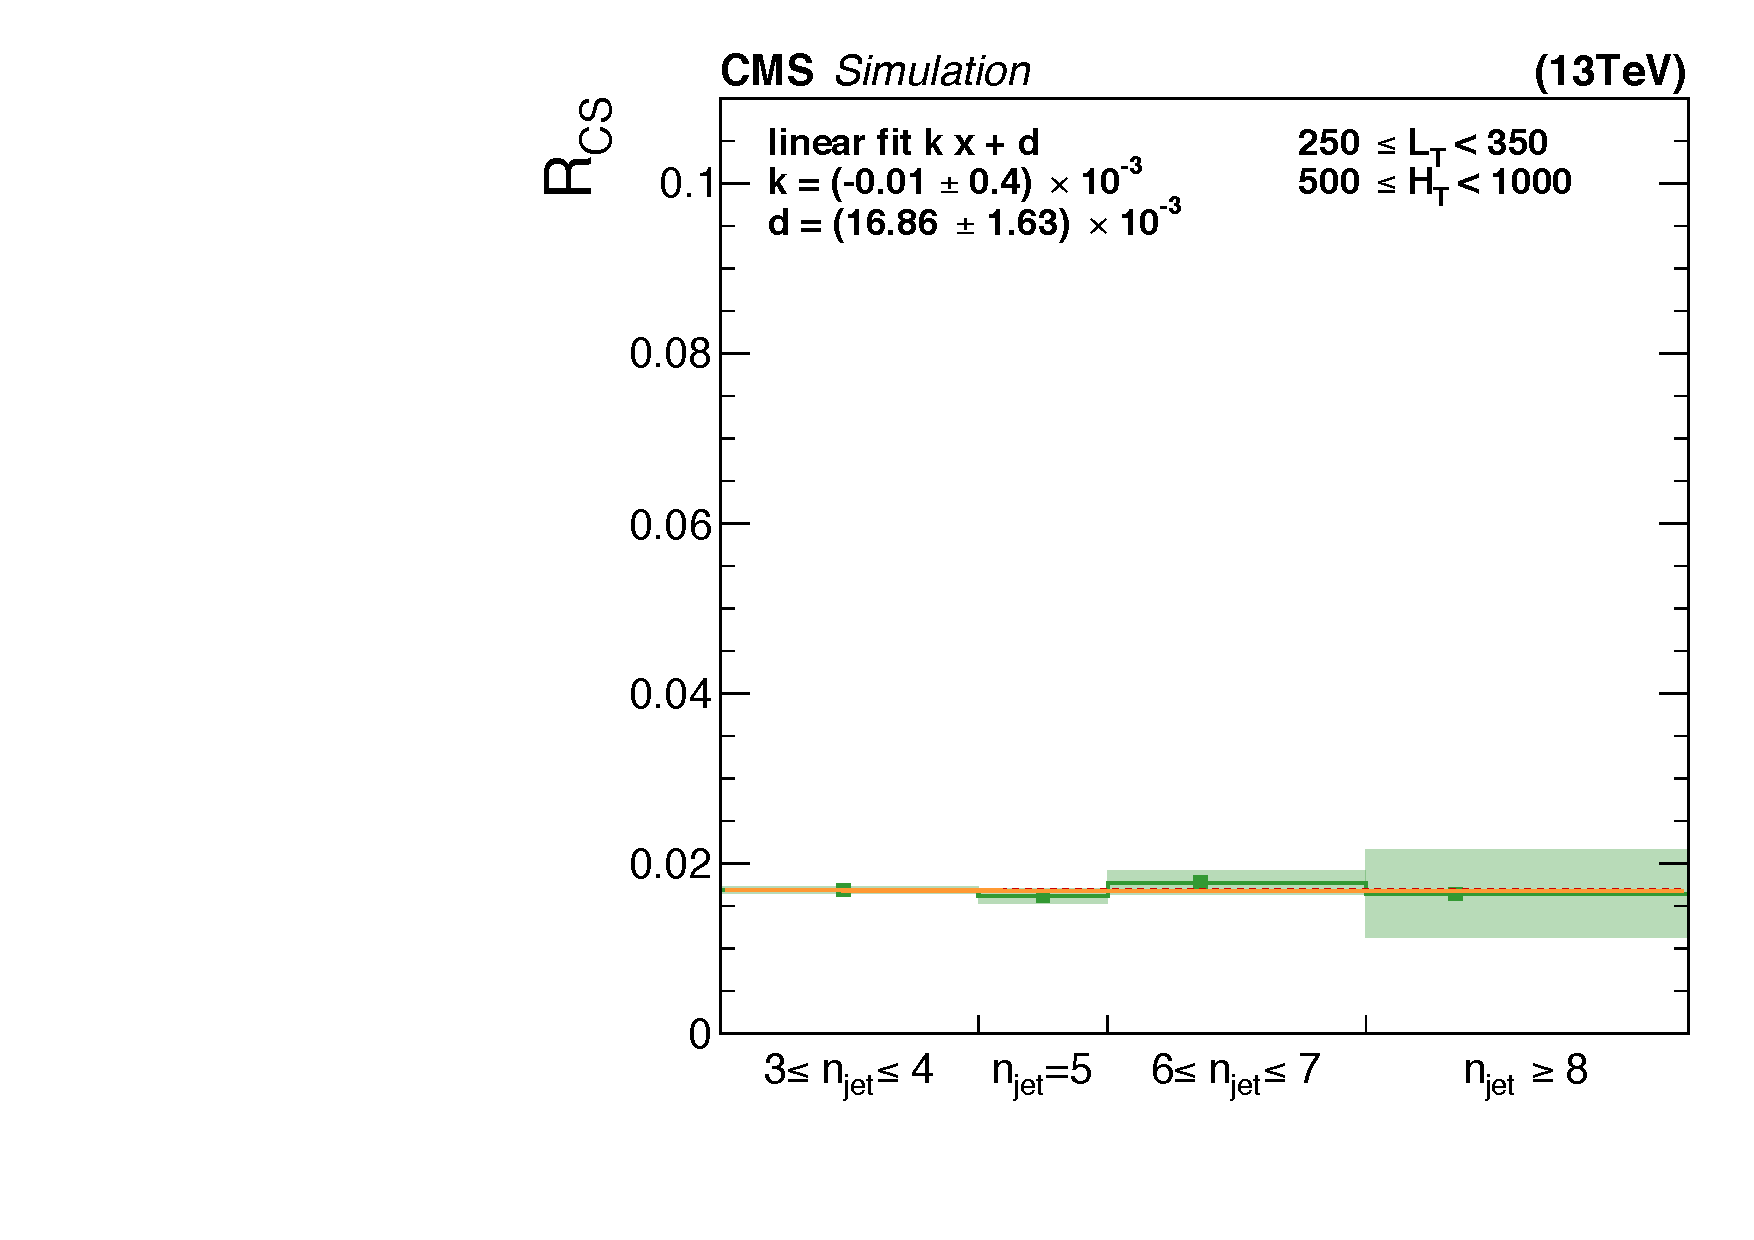
\includegraphics[width=0.45 \textwidth]{Plots/analysis/RCS/st250-350_ht500-1000_njet8_nbtag0_Wjets_NegPdg_fit}
  \caption{ \label{RCS_dataMCw}  $\Rcs$ as a function of njet from simulation of $\wJets$ events (left), and data (right) in $\wJets$ sideband. }
  \end{center}
\end{figure*}
Fig. \ref{RCS_dataMCw} shows simulated (left) and measured(right) values for the first search bin which is $\njet =$5, $\LT \in$ [250,350] GeV and $\HT \in$ [500,1000] GeV. Again as in the $\ttbar$ case, residual differences between the $\Rcs$ in the side band and main band is calculated in simulation as a correction factor $\kappa$. This time only one $\kappa$ factor is used, due to the fact that the side band and main band regions are sharing the same requirement for number of b-tagged jets, which is zero. The $\kappa_w$ accounts for residual dependence of $\Rcs$ on the jet multiplicity and also covers variances between $\Rcs$ values in muon only channel to combined lepton final state. The $\kappa_w$ is calculated as:
\begin{equation}
\label{kappa_w}
\kappa_w = \frac{R^{MC}_{CS}(0b,\njet: MB,\wJets)}{R^{Corr, MC}_{CS}(0b,\njet \in [3,4],\mu)}.
\end{equation}
Then the resultant $\Rcs$ is described as:
\begin{equation}
R^{W}_{CS}(0b,MB) = {\kappa_w}\cdot{R^{Corr. data}_{CS}(0b,\njet \in [3,4], \mu)}.
\end{equation}
Fig. \ref{fig:kappaW} shows the $\kappa_w$ values in the lower panel and $\Rcs$ values went into this calculation in the upper panel. In two kinematically extreme bins of high $\LT$ and low $\HT$ the Rcs values are different from the bulk but the SB follows the MB, therefore, $\kappa$ values are still compatible with 1.
\begin{figure*}[!hbt]
    \begin{center}
 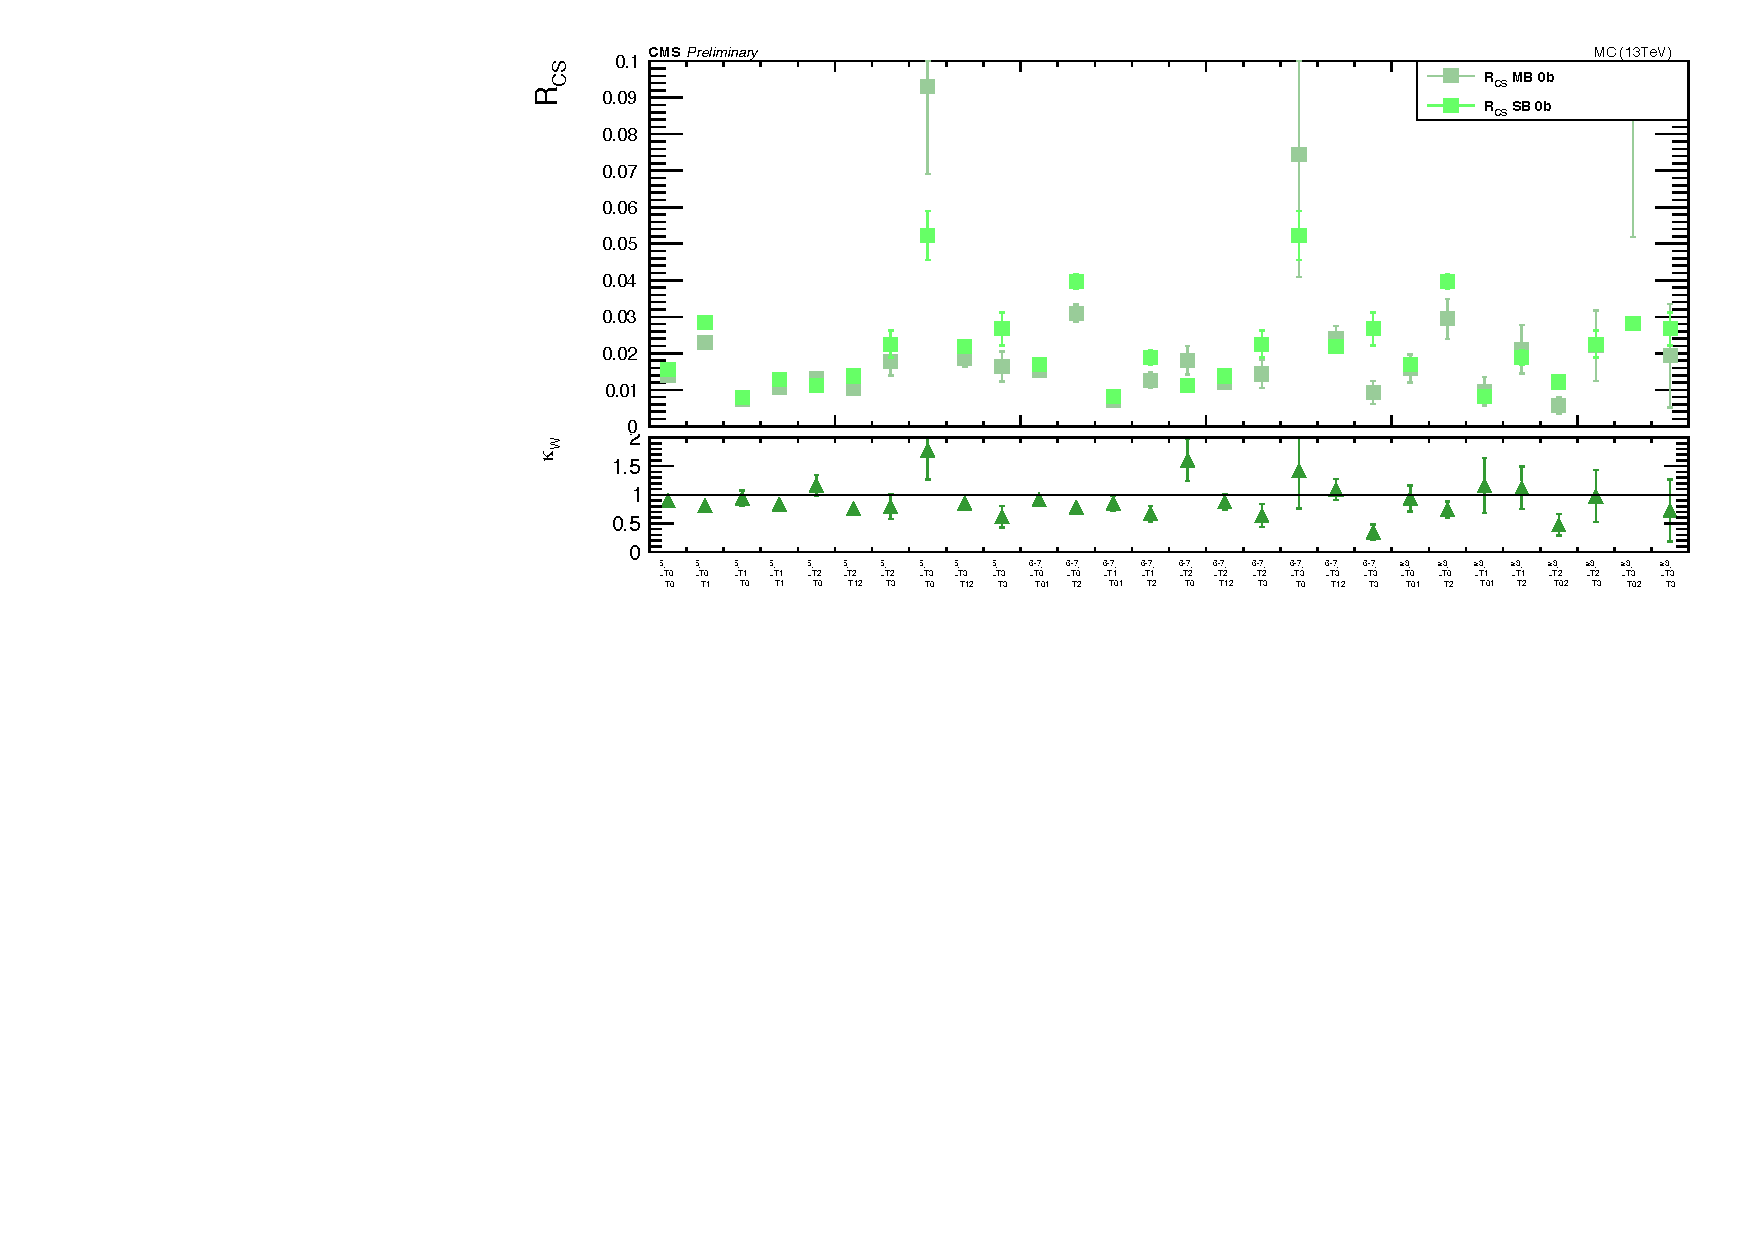
\includegraphics[width=1. \textwidth]{Plots/analysis/RCS/Spring16_templates_SR_Moriond2017_Summer16_lep_data_Kappa_W}
  \caption{ \label{fig:kappaW}  $\Rcs$ values went into $\kappa_w$(lower panel) calculation is shown.}
  \end{center}
\end{figure*}
\section{Validation of the background estimation}
\label{sec:Val}
Validation of the background estimation method is performed in events where there are four jets and zero b-tagged jets.
This region is a part of the $\wJets$ sideband of the main estimation and it is dominated by the SM background events. Consequently, in the validation, to perform the $\wJets$ prediction, only three jets region is used as the side band. The $\ttJets$ sideband remains unchanged since it is not used as the validation search region. Fig. \ref{kappaVal} presents the kappa values calculated for the validation.
\begin{figure*}[!hbt]
    \begin{center}
 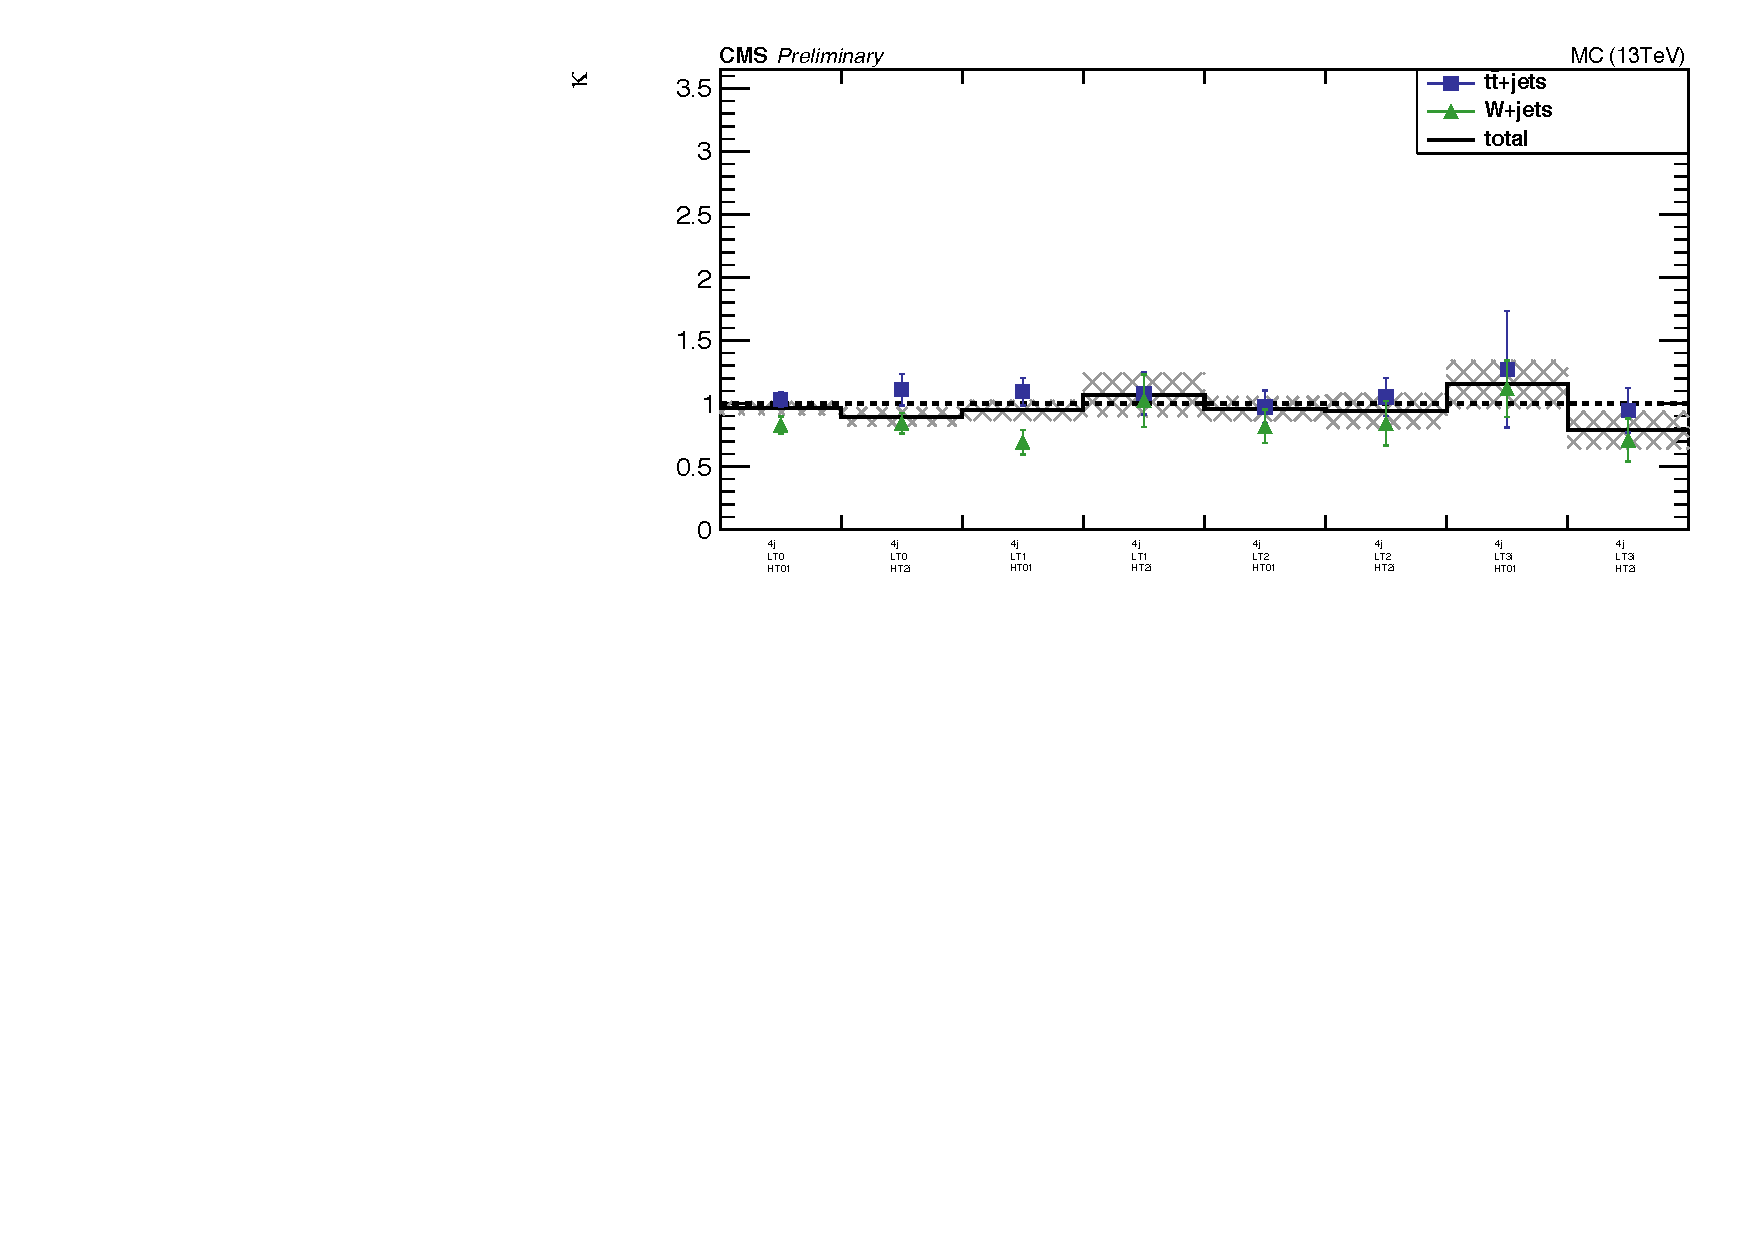
\includegraphics[width=0.8 \textwidth]{Plots/analysis/RCS/Spring16_templates_validation_4j_Moriond2017_lep_data_Kappa}
  \caption{ \label{kappaVal}  $\kappa_w$ and $\kappa_{\ttbar}$ correction factors are shown. The total $\kappa$, which is represented with black line, shows the ratio of prediction to the simulation. The shaded area displays the uncertainty coming from simulation statistics.}
  \end{center}
\end{figure*}
The results of the validation as well as the main prediction will be presented in Sec. \ref {sec:ResVal} after the discussion of the systematic uncertainties. 